\section{缩放本地多模态模型}

在本节中,我们呈现了本地多模态模型的缩放规律研究,考察了不同的架构选择~\cref{sec:scaling_laws_early},探索了不同的数据混合方式~\cref{sec:scaling_data_mix},分析了后期融合和早期融合NMMs之间的实际权衡,并比较了本地预训练和持续预训练NMMs的性能~\cref{sec:native_vs_continual}。

\cpar{设置。} 我们训练的模型参数范围从0.3B到4B,缩放宽度,同时保持深度不变。对于较小的训练标记预算,我们将预热阶段减少到1K步,而对于较大的预算,则保持5K步。
根据~\citet{hagele2024scaling},模型使用恒定学习率进行训练,然后使用逆平方根调度器进入冷却阶段。冷却阶段占总步骤的20\%,这些步骤在恒定学习率下进行。为了估算\Cref{eq:scaling_laws}中的缩放系数,我们应用了L-BFGS算法~\citep{lbfgs}和Huber损失~\citep{Huber1992}($\delta = 10^{-3}$),并在初始化范围上进行网格搜索。

\begin{table}[h!]
    \begin{minipage}[b]{1\linewidth}
        \centering
        \setlength{\tabcolsep}{24pt}
        \renewcommand{\arraystretch}{1}
        \resizebox{1\linewidth}{!}{
        \begin{tabular}{c c c c c}
             \grayrow $L \propto E+\frac{1}{N^{\alpha}}+\frac{1}{D^{\beta}}$ & $N \propto C^a$ & $D \propto C^b$ & $L \propto C^c$ & $D \propto N^d$ \\
        \end{tabular}}
      \label{tab:power_laws}
      \vspace{-3mm}
    \end{minipage}
    \begin{minipage}[b]{1\linewidth}
        \centering
        \setlength{\tabcolsep}{8pt}
        \renewcommand{\arraystretch}{1}
        \resizebox{1\linewidth}{!}{
        \begin{tabular}{lccccccccc}
            Model & Data & E & $\alpha$ & $\beta$ & a & b  & c & d \\ %
            \shline
            GPT3 \citep{brown2020language} & Text &  -- & -- & -- & -- & -- & -0.048 & \\% & 1.7 \\
            Chinchilla \citep{hoffmann2022training} & Text &  1.693 & 0.339 & 0.285 & 0.46 & 0.54 & -- & \\%& 20 \\
            \midrule
            \multirow{4}{*}{NMM (early-fusion)} & Text &  2.222 & 0.308 & 0.338 & 0.525 & 0.477     & -0.042 & 0.909 \\%& 58.35\\
            & Image-Caption & 1.569 & 0.311 & 0.339 & 0.520 & 0.479 & -0.061 & 0.919 \\% & 72.21\\
            & Interleaved & 1.966 & 0.297 & 0.338 & 0.532 & 0.468     & -0.046 & 0.879 \\%& 57.74\\
            & AVG & 1.904 & 0.301 & 0.335 & 0.526 & 0.473 & -0.049 & 0.899 \\% & 64.05\\
            \midrule
            NMM (late-fusion) & AVG &  1.891 & 0.290 & 0.338 & 0.636 & 0.462 & -0.049 & 0.673 \\%& 46.19\\
            \midrule
            \edit{Sparse NMM (early-fusion)} & AVG & 2.158  & 0.710 & 0.372 & 0.361  & 0.656 & -0.047 & 1.797 \\%& 46.19\\
        \end{tabular}%
        } \caption{\textbf{Scaling laws for native multimodal models}. We report the
        scaling laws results for early and late fusion models. We fit the scaling laws for different target data types as well as their average loss (AVG).
        }
        \label{tab:early_vs_late_coeffs}
    \end{minipage}
    \vspace{-3mm}
\end{table}


\begin{figure*}[t!]
    \centering
    \captionsetup{type=figure}
    \begin{subfigure}[t]{0.33\linewidth}
        \begin{tikzpicture}
    \begin{axis}[
        legend pos=north east,
        grid=major, %
        grid style={line width=.1pt, draw=gray!30}, %
        major grid style={line width=.2pt,draw=gray!50},
        minor tick num=2,
        axis x line*=bottom,
        axis y line*=left,
        xmode=log, %
        log basis x=10, %
        height=1.7in,
        width=1.05\linewidth,
        ylabel style={align=center, font=\scriptsize, yshift=-1ex},
        xlabel style={font=\scriptsize},
        ylabel={\footnotesize{Validation Loss}},
        xlabel={\scriptsize{FLOPs}},
        title=\footnotesize{Image-Caption},
        yticklabel style={font=\scriptsize, /pgf/number format/fixed, /pgf/number format/precision=1},
        xticklabel style={font=\scriptsize},
        mark options={solid},
        legend style={cells={align=left}, font=\footnotesize, text=black}, %
        legend columns=6, %
        legend cell align={left},
        legend to name=sharedlegend,
    ]
    \addplot[legend late_0_2b style] plot coordinates {
        (8.1e+19, 2.967)
        (1.62e+20, 2.874)
        (3.24e+20, 2.797)
        (6.48e+20, 2.728)

    };

    \addplot[legend late_0_4b style] plot coordinates {
        (1.37e+20, 2.869)
        (2.74e+20, 2.771)
        (5.48e+20, 2.695)
        (1.1e+21, 2.626)

    };

    \addplot[legend late_0_9b style] plot coordinates {
        (2.78e+20, 2.734)
        (5.56e+20, 2.629)
        (1.11e+21, 2.541)
        (2.22e+21, 2.467)

    };



    \addplot[legend late_2_2b style] plot coordinates {
        (1.34e+21, 2.466)
        (2.69e+21, 2.367)
        (5.37e+21, 2.287)
        (8.06e+21, 2.255)
    };

        







    \addplot[legend early_0_2b style] plot coordinates {
        (8.25e+19, 2.95)
        (1.65e+20, 2.865)
        (3.3e+20, 2.781)
        (6.6e+20, 2.715)


    };
    \addplot[legend early_0_4b style] plot coordinates {
        (1.39e+20, 2.852)
        (2.78e+20, 2.755)
        (5.57e+20, 2.663)
        (1.11e+21, 2.596)


    };
    \addplot[legend early_0_9b style] plot coordinates {
        (2.8e+20, 2.716)
        (5.59e+20, 2.598)
        (1.12e+21, 2.495)
        (2.24e+21, 2.425)


    };

        
    \addplot[legend early_2_2b style] plot coordinates {
        (1.37e+21, 2.455)
        (2.74e+21, 2.352)
        (5.47e+21, 2.279)
        (8.21e+21, 2.242)
    };
        
    

    \end{axis}
\end{tikzpicture}
    \end{subfigure}
    \begin{subfigure}[t]{0.32\linewidth}
        \begin{tikzpicture}
    \begin{axis}[
        legend pos=north east,
        grid=major,
        grid style={line width=.1pt, draw=gray!30},
        major grid style={line width=.2pt,draw=gray!50},
        minor tick num=2,
        axis x line*=bottom,
        axis y line*=left,
        xmode=log,
        log basis x=10,
        height=1.7in,
        width=1.05\linewidth,
        ylabel style={align=center, font=\scriptsize, yshift=-1ex},
        xlabel style={font=\scriptsize},
        xlabel={\scriptsize{FLOPs}},
        title=\footnotesize{Interleaved},
        yticklabel style={font=\scriptsize, /pgf/number format/fixed, /pgf/number format/precision=1},
        xticklabel style={font=\scriptsize},
        mark options={solid},
        legend style={cells={align=left}, font=\footnotesize, text=black},
        legend columns=6,
        legend cell align={left},
        legend to name=sharedlegend,
    ]

\addplot[legend late_0_2b style] plot coordinates {
        (8.1e+19, 3.113)
        (1.62e+20, 3.044)
        (3.24e+20, 2.988)
        (4.86e+20, 2.959)
        (6.48e+20, 2.94)
    };

    \addplot[legend late_0_4b style] plot coordinates {
        (1.37e+20, 3.013)
        (2.74e+20, 2.942)
        (5.48e+20, 2.883)
        (8.22e+20, 2.853)
        (1.1e+21, 2.833)

    };

    \addplot[legend late_0_9b style] plot coordinates {
        (2.78e+20, 2.899)
        (5.56e+20, 2.811)
        (1.11e+21, 2.741)
        (2.22e+21, 2.685)

    };
    \addlegendentry{Late-1B}

\addplot[legend late_2_2b style] plot coordinates {
        (1.34e+21, 2.697)
        (2.69e+21, 2.621)
        (4.03e+21, 2.58)
        (5.37e+21, 2.557)
        (8.06e+21, 2.527)

    };
    \addlegendentry{Late-2.4B}

\addplot[legend early_0_2b style] plot coordinates {
        (8.25e+19, 3.094)
        (1.65e+20, 3.022)
        (3.3e+20, 2.967)
        (4.95e+20, 2.939)
        (6.6e+20, 2.921)
    };

    \addplot[legend early_0_4b style] plot coordinates {
        (1.39e+20, 2.998)
        (2.78e+20, 2.927)
        (5.57e+20, 2.866)
        (8.35e+20, 2.836)
        (1.11e+21, 2.817)
    };

    \addplot[legend early_0_9b style] plot coordinates {
        (2.8e+20, 2.885)
        (5.59e+20, 2.795)
        (1.12e+21, 2.726)
        (2.24e+21, 2.669)
    };

    \addlegendentry{Early-0.9B}

\addplot[legend early_2_2b style] plot coordinates {
        (1.37e+21, 2.685)
        (2.74e+21, 2.61)
        (4.1e+21, 2.572)
        (5.47e+21, 2.542)
        (8.21e+21, 2.514)

    };
    \addlegendentry{Early-2.2B}

\end{axis}
\end{tikzpicture}

    \end{subfigure}
    \begin{subfigure}[t]{0.32\linewidth}
    \begin{tikzpicture}
    \begin{axis}[
        legend pos=north east,
        grid=major,
        grid style={line width=.1pt, draw=gray!30},
        major grid style={line width=.2pt,draw=gray!50},
        minor tick num=2,
        axis x line*=bottom,
        axis y line*=left,
        xmode=log,
        log basis x=10,
        height=1.7in,
        width=1.05\linewidth,
        ylabel style={align=center, font=\scriptsize, yshift=-1ex},
        xlabel style={font=\scriptsize},
        xlabel={\scriptsize{FLOPs}},
        title=\footnotesize{Text-only},
        yticklabel style={font=\scriptsize, /pgf/number format/fixed, /pgf/number format/precision=1},
        xticklabel style={font=\scriptsize},
        mark options={solid},
        legend style={cells={align=left}, font=\scriptsize, text=black},
        legend columns=4,
        legend cell align={left},
        legend to name=sharedlegend,
    ]

    \addplot[legend late_0_2b style] plot coordinates {
        (8.1e+19, 3.349)
        (1.62e+20, 3.281)
        (3.24e+20, 3.226)
        (4.86e+20, 3.197)
        (6.48e+20, 3.179)

    };
    \addlegendentry{Late-289M}

    \addplot[legend late_0_4b style] plot coordinates {
        (1.37e+20, 3.249)
        (2.74e+20, 3.177)
        (5.48e+20, 3.12)
        (8.22e+20, 3.09)
        (1.1e+21, 3.071)
    };
    \addlegendentry{Late-494M}

\addplot[legend late_0_9b style] plot coordinates {
        (2.78e+20, 3.134)
        (5.56e+20, 3.045)
        (1.11e+21, 2.976)
        (1.67e+21, 2.941)
        (2.22e+21, 2.92)

    };
    \addlegendentry{Late-1B}

\addplot[legend late_2_2b style] plot coordinates {
        (1.34e+21, 2.936)
        (2.69e+21, 2.859)
        (5.37e+21, 2.798)
        (8.06e+21, 2.765)

    };
    \addlegendentry{Late-2.4B}

\addplot[legend early_0_2b style] plot coordinates {
        (8.25e+19, 3.328)
        (1.65e+20, 3.259)
        (3.3e+20, 3.203)
        (4.95e+20, 3.175)
        (6.6e+20, 3.157)
    };
    \addlegendentry{Early-275M}

\addplot[legend early_0_4b style] plot coordinates {
        (1.39e+20, 3.232)
        (2.78e+20, 3.161)
        (5.57e+20, 3.103)
        (8.35e+20, 3.073)
        (1.11e+21, 3.054)
    };
    \addlegendentry{Early-464M}

    \addplot[legend early_0_9b style] plot coordinates {
        (2.8e+20, 3.119)
        (5.59e+20, 3.03)
        (1.12e+21, 2.961)
        (1.68e+21, 2.926)
        (2.24e+21, 2.904)
    };
    \addlegendentry{Early-932M}

\addplot[legend early_2_2b style] plot coordinates {
        (1.37e+21, 2.923)
        (2.74e+21, 2.846)
        (5.47e+21, 2.784)
        (8.21e+21, 2.752)
    };
    \addlegendentry{Early-2.28B}

\end{axis}
\end{tikzpicture}

    \end{subfigure}
    \begin{center}
        \ref{sharedlegend}
    \end{center}
    \caption{\textbf{早期融合与晚期融合:缩放训练浮点运算。} 我们比较了在缩放模型参数数量和训练词元数量时的早期融合模型和晚期融合模型。总体而言,早期融合显示出轻微的优势,尤其是在较小的模型规模下,随着参数数量的增加,差距减小 $N$ 。}
    \label{fig:early_vs_late_scaleflops}
    \vspace{3mm}
\end{figure*}

\vspace{-0.5cm}
\subsection{NMM 的缩放法则}
\label{sec:scaling_laws_early}

\cpar{早期融合与后期融合模型的缩放法则。}
\Cref{fig:early_vs_late_scaleflops_3d}~(左) 展示了早期融合 NMM 在交错数据、图文配对数据和纯文本数据上的最终损失均值。最低损失前沿遵循 FLOPs 的幂律函数。拟合该幂律得到表达式 $L \propto C^{-0.049}$,表明随着计算量增加,模型性能的提升速率。当分别按数据类型(如图文配对、交错、文本)分析缩放法则时,可以观察到指数有所差异(见 \cref{tab:early_vs_late_coeffs})。例如,在图文配对数据上模型获得更高的提升速率 $(L \propto C^{-0.061})$,而在交错文档上为 $(L \propto C^{-0.046})$。

为了将损失建模为训练 token 数 $D$ 和模型参数量 $N$ 的函数,我们对 \cref{eq:scaling_laws} 中的参数化函数进行拟合,得到缩放指数 $\alpha = 0.301$ 和 $\beta = 0.335$。这两个指数分别描述了随着模型参数量和训练 token 数增加时的性能提升速率。假设计算量 $C$ 与 $N$ 和 $D$ 成线性关系(即 $C \propto ND$),我们推导了模型参数与计算预算之间的关系法则(详见 \cref{app:scaling_laws})。具体而言,对于给定的计算预算 $C$,我们在对数间距的 $D$ 值下计算对应的模型大小 $N$,并确定能够最小化损失的参数数量 $N_{opt}$。在不同 FLOPs 值上重复此过程,生成 $(C, N_{opt})$ 数据集,并拟合一个幂律函数来预测最优模型大小与计算量之间的关系:$N^* \propto C^{0.526}.$

类似地,我们拟合幂律函数来估计最优训练数据集大小与计算量和模型大小之间的关系:
\[
D_{opt} \propto C^{0.473}, \quad D_{opt} \propto N^{0.899}.
\]
这些关系使实践者能够在固定计算预算下确定最优模型规模和数据集大小。按数据类型分析时,我们发现交错数据相比图文配对数据更受益于更大的模型规模($a=0.532$ 对比 $a=0.520$),而在训练 token 数方面则表现出相反的趋势。

\begin{figure*}[t!]
    \centering
    \captionsetup{type=figure}
    \begin{subfigure}[t]{0.24\linewidth}
        \begin{tikzpicture}
    \begin{axis}[
        grid=both,
        grid style={line width=.1pt, draw=gray!10},
        major grid style={line width=.2pt,draw=gray!50},
        minor tick num=2,
        axis x line*=bottom,
        axis y line*=left,
        xmode=log,
        log basis x=10,
        xtick={
            1E+19,
            1E+20,
            1E+21,
            1E+22
        },
        xmin=2E+18,
        xmax=2E+22,
        ymax=4.3,
        height=1.7in,
        width=1.15\linewidth,
        ylabel style={align=center, font=\scriptsize, yshift=-1ex},
        xlabel style={font=\scriptsize},
        title={\footnotesize{\colorbox{blue!10}{45-45-10}}},
        ylabel={Validation Loss},
        xlabel={\scriptsize{FLOPs}},
        yticklabel style={font=\scriptsize},
        xticklabel style={font=\scriptsize},
        legend style={cells={align=left}, font=\scriptsize, fill opacity=0.7, fill=none,at={(-0.3,0.95)}, anchor=west, draw=none},
        legend cell align={left},
        mark options={solid},
    ]

\addplot[color=white, samples=50, domain=5e18:10e21, mark=none] {29.574*x^(-0.04919)};
    \addlegendentry{\scalebox{0.9}{$L = 29.574C^{-0.0492}$}};
    \addplot[color=black, samples=50, domain=5e18:10e21, forget plot] {29.574*x^(-0.04919)};

\addplot[legend early_0_2b style, mark size=1pt] plot coordinates {
        (4.13e+18, 3.9896666666666665)
        (8.25e+18, 3.5996666666666663)
        (1.24e+19, 3.468)
        (2.06e+19, 3.358333333333333)
        (4.13e+19, 3.2113333333333336)
        (6.19e+19, 3.1543333333333337)
        (8.25e+19, 3.124)
        (1.65e+20, 3.048666666666667)
        (3.3e+20, 2.9836666666666667)
        (4.95e+20, 2.9506666666666668)
        (6.6e+20, 2.9309999999999996)
    };
    \addplot[legend early_0_4b style, mark size=1pt] plot coordinates {
        (6.96e+18, 3.887333333333333)
        (1.39e+19, 3.5203333333333333)
        (2.09e+19, 3.3823333333333334)
        (3.48e+19, 3.2710000000000004)
        (6.96e+19, 3.1170000000000004)
        (1.04e+20, 3.058666666666667)
        (1.39e+20, 3.0273333333333334)
        (2.78e+20, 2.9476666666666667)
        (5.57e+20, 2.877333333333333)
        (8.35e+20, 2.8433333333333333)
        (1.11e+21, 2.8223333333333334)
        (1.39e+21, 2.8063333333333333)
        (1.67e+21, 2.7936666666666667)
    };
    \addplot[legend early_0_9b style, mark size=1pt] plot coordinates {
        (1.4e+19, 3.955)
        (2.8e+19, 3.465)
        (4.19e+19, 3.3143333333333334)
        (6.99e+19, 3.2099999999999995)
        (1.4e+20, 3.0193333333333334)
        (2.1e+20, 2.9483333333333337)
        (2.8e+20, 2.9066666666666663)
        (5.59e+20, 2.807666666666666)
        (1.12e+21, 2.7273333333333327)
        (1.68e+21, 2.688333333333333)
        (2.24e+21, 2.666)
        (2.8e+21, 2.6466666666666665)
        (3.36e+21, 2.635333333333333)
    };

    \addplot[legend early style, mark size=1pt] plot coordinates {
        (2.44e+19, 3.859666666666667)
        (4.88e+19, 3.3973333333333335)
        (7.32e+19, 3.25)
        (1.22e+20, 3.1323333333333334)
        (2.44e+20, 2.9466666666666668)
        (3.66e+20, 2.875666666666667)
        (4.88e+20, 2.8206666666666664)
        (9.76e+20, 2.7246666666666672)
        (1.95e+21, 2.646666666666667)
        (2.93e+21, 2.6056666666666666)
        (3.9e+21, 2.582333333333333)
        (4.88e+21, 2.562)
        (5.86e+21, 2.548666666666666)
    };

    \addplot[legend early_2_2b style, mark size=1pt] plot coordinates {
        (3.42e+19, 3.859666666666667)
        (6.84e+19, 3.3973333333333335)
        (1.03e+20, 3.2503333333333333)
        (1.71e+20, 3.098333333333333)
        (3.42e+20, 2.9156666666666666)
        (5.13e+20, 2.8396666666666666)
        (6.84e+20, 2.7913333333333337)
        (1.37e+21, 2.687666666666667)
        (2.74e+21, 2.6026666666666665)
        (4.1e+21, 2.562)
        (5.47e+21, 2.5349999999999997)
        (6.84e+21, 2.5146666666666664)
        (8.21e+21, 2.502666666666667)
    };
    \addplot[legend early_3_3b style, mark size=1pt] plot coordinates {
        (5.03e+19, 3.746333333333333)
        (1.01e+20, 3.324)
        (1.51e+20, 3.1786666666666665)
        (2.52e+20, 3.0766666666666667)
        (5.03e+20, 2.8836666666666666)
        (7.55e+20, 2.8029999999999995)
        (1.01e+21, 2.7550000000000003)
        (2.01e+21, 2.6473333333333335)
        (4.02e+21, 2.5583333333333336)
        (6.04e+21, 2.5163333333333333)
        (8.05e+21, 2.4886666666666666)
        (1.01e+22, 2.466666666666667)
    };

\end{axis}
\end{tikzpicture}

    \end{subfigure}
    \begin{subfigure}[t]{0.24\linewidth}
        \begin{tikzpicture}
    \begin{axis}[
        legend pos=north east,
        grid=both,
        grid style={line width=.1pt, draw=gray!10},
        major grid style={line width=.2pt,draw=gray!50},
        minor tick num=2,
        axis x line*=bottom,
        axis y line*=left,
        xmode=log,
        log basis x=10,
        xtick={
            1E+19,
            1E+20,
            1E+21,
            1E+22
        },
        xmin=2E+18,
        xmax=2E+22,
        ymax=4.3,
        height=1.7in,
        width=1.15\linewidth,
        ylabel style={align=center, font=\scriptsize, yshift=-1ex},
        xlabel style={font=\scriptsize},
        title=\footnotesize{\colorbox{green!10}{40-20-40}},
        xlabel={\scriptsize{FLOPs}},
        yticklabel style={font=\scriptsize},
        xticklabel style={font=\scriptsize},
        legend style={cells={align=left}, font=\scriptsize, fill opacity=0.7, fill=none,  draw=none,at={(-0.3,0.95)}, anchor=west},
        legend cell align={left},
        mark options={solid},
    ]

    \addplot[color=white, samples=50, domain=5e18:10e21, mark=none] {29.574*x^(-0.04919)};
    \addlegendentry{\scalebox{0.9}{$L = 28.590C^{-0.0486}$}};
    \addplot[color=black, samples=50, domain=5e18:10e21] {28.589490029895153*x^(-0.048605069004824725)};

    \addplot[legend early_0_2b style, mark size=1pt] plot coordinates {
        (4.13e+18, 3.968)
        (8.25e+18, 3.563)
        (1.24e+19, 3.4296666666666664)
        (2.06e+19, 3.3236666666666665)
        (4.13e+19, 3.203)
        (6.19e+19, 3.1486666666666667)
        (8.25e+19, 3.1169999999999995)
        (1.65e+20, 3.0446666666666666)
        (3.3e+20, 2.9906666666666673)
        (4.95e+20, 2.9633333333333334)
        (6.6e+20, 2.9456666666666664)
    };
    \addplot[legend early_0_4b style, mark size=1pt] plot coordinates {
        (6.96e+18, 3.8580000000000005)
        (1.39e+19, 3.471)
        (2.09e+19, 3.3443333333333336)
        (3.48e+19, 3.2196666666666665)
        (6.96e+19, 3.097666666666667)
        (1.04e+20, 3.0393333333333334)
        (1.39e+20, 3.011333333333333)
        (2.78e+20, 2.935333333333333)
        (5.57e+20, 2.871)
        (8.35e+20, 2.8386666666666667)
        (1.11e+21, 2.8190000000000004)
        (1.39e+21, 2.8030000000000004)
        (1.67e+21, 2.7913333333333337)
    };
    \addplot[legend early_0_9b style, mark size=1pt] plot coordinates {
        (1.4e+19, 3.9250000000000003)
        (2.8e+19, 3.426666666666667)
        (4.19e+19, 3.2733333333333334)
        (6.99e+19, 3.1326666666666667)
        (1.4e+20, 2.9979999999999998)
        (2.1e+20, 2.9246666666666665)
        (2.8e+20, 2.8943333333333334)
        (5.59e+20, 2.8070000000000004)
        (1.12e+21, 2.7283333333333335)
        (1.68e+21, 2.6886666666666668)
        (2.24e+21, 2.666)
        (2.8e+21, 2.6476666666666664)
        (3.36e+21, 2.636)
    };

    \addplot[legend early style, mark size=1pt] plot coordinates {
        (2.44e+19, 3.846)
        (4.88e+19, 3.3570000000000007)
        (7.32e+19, 3.207333333333333)
        (1.22e+20, 3.0636666666666668)
        (2.44e+20, 2.9229999999999996)
        (3.66e+20, 2.848666666666667)
        (4.88e+20, 2.8166666666666664)
        (9.76e+20, 2.7126666666666672)
        (1.95e+21, 2.632)
        (2.93e+21, 2.592333333333333)
        (3.9e+21, 2.569666666666667)
        (4.88e+21, 2.5516666666666667)
        (5.86e+21, 2.538)
    };

    \addplot[legend early_2_2b style, mark size=1pt] plot coordinates {
        (3.42e+19, 3.771333333333333)
        (6.84e+19, 3.317)
        (1.03e+20, 3.1679999999999997)
        (1.71e+20, 3.025)
        (3.42e+20, 2.887)
        (5.13e+20, 2.8106666666666666)
        (6.84e+20, 2.781333333333334)
        (1.37e+21, 2.6756666666666664)
        (2.74e+21, 2.593666666666666)
        (4.1e+21, 2.5526666666666666)
        (5.47e+21, 2.526666666666667)
        (6.84e+21, 2.5093333333333336)
        (8.21e+21, 2.494333333333333)
    };
    \addplot[legend early_3_3b style, mark size=1pt] plot coordinates {
        (5.03e+19, 3.7276666666666665)
        (1.01e+20, 3.2793333333333337)
        (1.51e+20, 3.1359999999999997)
        (2.52e+20, 2.9949999999999997)
        (5.03e+20, 2.879)
        (7.55e+20, 2.787333333333333)
        (1.01e+21, 2.738666666666667)
        (2.01e+21, 2.6276666666666664)
        (4.02e+21, 2.5466666666666664)
        (6.04e+21, 2.5180000000000002)
        (8.05e+21, 2.4789999999999996)
        (1.01e+22, 2.456)
        (1.21e+22, 2.4516666666666667)
    };

\end{axis}
\end{tikzpicture}

    \end{subfigure}
    \begin{subfigure}[t]{0.24\linewidth}
        \begin{tikzpicture}
    \begin{axis}[
        legend pos=north east,
        grid=both,
        grid style={line width=.1pt, draw=gray!10},
        major grid style={line width=.2pt,draw=gray!50},
        minor tick num=2,
        axis x line*=bottom,
        axis y line*=left,
        xmode=log,
        log basis x=10,
        xtick={
            1E+19,
            1E+20,
            1E+21,
            1E+22
        },
        xmin=2E+18,
        xmax=2E+22,
        ymax=4.3,
        height=1.7in,
        width=1.15\linewidth,
        ylabel style={align=center, font=\scriptsize, yshift=-1ex},
        xlabel style={font=\scriptsize},
        title=\footnotesize{\colorbox{red!10}{30-30-40}},
        xlabel={\scriptsize{FLOPs}},
        yticklabel style={font=\scriptsize},
        xticklabel style={font=\scriptsize},
        legend style={cells={align=left}, font=\scriptsize, fill opacity=0.7, fill=none,  draw=none,at={(-0.3,0.95)}, anchor=west},
        legend cell align={left},
        mark options={solid},
    ]

    \addplot[color=white, samples=50, domain=5e18:10e21, mark=none] {29.574*x^(-0.04919)};
    \addlegendentry{\scalebox{0.9}{$L = 25.623C^{-0.0463}$}};
    \addplot[color=black, samples=50, domain=5e18:10e21] {25.622649599876997*x^(-0.04634327762259929)};

    \addplot[legend early_0_2b style, mark size=1pt] plot coordinates {
        (4.13e+18, 3.9586666666666672)
        (8.25e+18, 3.568)
        (1.24e+19, 3.402333333333333)
        (2.06e+19, 3.235666666666667)
        (4.13e+19, 3.200333333333333)
        (6.19e+19, 3.1493333333333333)
        (8.25e+19, 3.0506666666666664)
        (1.65e+20, 2.9996666666666663)
        (3.3e+20, 2.9996666666666663)
        (4.95e+20, 2.969666666666667)
        (6.6e+20, 2.9486666666666665)
    };
    \addplot[legend early_0_4b style, mark size=1pt] plot coordinates {
        (6.96e+18, 3.8503333333333334)
        (1.39e+19, 3.472)
        (2.09e+19, 3.3366666666666664)
        (3.48e+19, 3.2273333333333336)
        (6.96e+19, 3.095)
        (1.04e+20, 3.0406666666666666)
        (1.39e+20, 3.016)
        (2.78e+20, 2.9373333333333336)
        (5.57e+20, 2.8753333333333337)
        (8.35e+20, 2.8433333333333333)
        (1.11e+21, 2.8223333333333334)
        (1.39e+21, 2.8073333333333337)
        (1.67e+21, 2.797333333333333)
    };
    \addplot[legend early_0_9b style, mark size=1pt] plot coordinates {
        (1.4e+19, 3.8346666666666667)
        (2.8e+19, 3.3586666666666662)
        (4.19e+19, 3.202)
        (6.99e+19, 3.1340000000000003)
        (1.4e+20, 2.9949999999999997)
        (2.1e+20, 2.9273333333333333)
        (2.8e+20, 2.8930000000000002)
        (5.59e+20, 2.8053333333333335)
        (1.12e+21, 2.728333333333333)
        (1.68e+21, 2.692666666666667)
        (2.24e+21, 2.667666666666667)
        (2.8e+21, 2.6496666666666666)
        (3.36e+21, 2.639666666666667)
    };

    \addplot[legend early style, mark size=1pt] plot coordinates {
        (2.44e+19, 3.8346666666666667)
        (4.88e+19, 3.3586666666666662)
        (7.32e+19, 3.202)
        (1.22e+20, 3.063333333333334)
        (2.44e+20, 2.9196666666666666)
        (3.66e+20, 2.8503333333333334)
        (4.88e+20, 2.8196666666666665)
        (9.76e+20, 2.719)
        (1.95e+21, 2.6359999999999997)
        (2.93e+21, 2.6)
        (3.9e+21, 2.574)
        (4.88e+21, 2.554)
        (5.86e+21, 2.5436666666666667)
    };

    \addplot[legend early_2_2b style, mark size=1pt] plot coordinates {
        (3.42e+19, 3.755333333333333)
        (6.84e+19, 3.311)
        (1.03e+20, 3.159333333333333)
        (1.71e+20, 3.025)
        (3.42e+20, 2.8770000000000002)
        (5.13e+20, 2.8089999999999997)
        (6.84e+20, 2.781333333333333)
        (1.37e+21, 2.679)
        (2.74e+21, 2.595)
        (4.1e+21, 2.5536666666666665)
        (5.47e+21, 2.5283333333333333)
        (6.84e+21, 2.5066666666666664)
        (8.21e+21, 2.4953333333333334)
    };
    \addplot[legend early_3_3b style, mark size=1pt] plot coordinates {
        (5.03e+19, 3.7100000000000004)
        (1.01e+20, 3.276666666666667)
        (1.51e+20, 3.1300000000000003)
        (2.52e+20, 2.997)
        (5.03e+20, 2.84)
        (7.55e+20, 2.768333333333333)
        (1.01e+21, 2.7436666666666665)
        (2.01e+21, 2.6343333333333336)
        (4.02e+21, 2.5513333333333335)
        (6.04e+21, 2.5086666666666666)
        (8.05e+21, 2.483)
        (1.01e+22, 2.4616666666666664)
    };

\end{axis}
\end{tikzpicture}

    \end{subfigure}
    \begin{subfigure}[t]{0.24\linewidth}
        
\begin{tikzpicture}
    \begin{axis}[
        legend pos=north east,
        grid=both,
        grid style={line width=.1pt, draw=gray!10},
        major grid style={line width=.2pt,draw=gray!50},
        minor tick num=2,
        axis x line*=bottom,
        axis y line*=left,
        xmode=log, %
        log basis x=10, %
        xtick={
            1E+19,
            1E+20,
            1E+21,
            1E+22
        },
        xmin=2E+18,
        xmax=2E+22,
        ymax=4.3,
        height=1.7in,
        width=1.15\linewidth,
        ylabel style={align=center, font=\scriptsize, yshift=-1ex},
        xlabel style={font=\scriptsize},
        title={\footnotesize{\colorbox{orange!10}{20-40-40}}},
        xlabel={\scriptsize{FLOPs}},
        yticklabel style={font=\scriptsize},
        xticklabel style={font=\scriptsize},
        legend style={cells={align=left}, font=\scriptsize, fill opacity=0.7, fill=none,  draw=none,at={(-0.3,0.95)}, anchor=west}, %
        legend cell align={left},
        mark options={solid},
    ]

    \addplot[color=white, samples=50, domain=5e18:10e21, mark=none] {29.574*x^(-0.04919)};
    \addlegendentry{\scalebox{0.9}{$L = 29.002C^{-0.0488}$}};
    \addplot[color=black, samples=50, domain=5e18:10e21] {29.002272950965768*x^(-0.04878835579770303)};

    \addplot[legend early_0_2b style, mark size=1pt] plot coordinates {
        (4.13e+18, 3.984666666666667)
        (8.25e+18, 3.592333333333334)
        (1.24e+19, 3.453333333333333)
        (2.06e+19, 3.3553333333333337)
        (4.13e+19, 3.2129999999999996)
        (6.19e+19, 3.1616666666666666)
        (8.25e+19, 3.1376666666666666)
        (1.65e+20, 3.0653333333333332)
        (3.3e+20, 3.0080000000000005)
        (4.95e+20, 2.9793333333333334)
        (6.6e+20, 2.9603333333333333)
    };
    \addplot[legend early_0_4b style, mark size=1pt] plot coordinates {
        (6.96e+18, 3.861333333333333)
        (1.39e+19, 3.4956666666666667)
        (2.09e+19, 3.361333333333333)
        (3.48e+19, 3.2516666666666665)
        (6.96e+19, 3.1056666666666666)
        (1.04e+20, 3.0546666666666664)
        (1.39e+20, 3.0293333333333337)
        (2.78e+20, 2.959)
        (5.57e+20, 2.9013333333333335)
        (8.35e+20, 2.8683333333333336)
        (1.11e+21, 2.8463333333333334)
        (1.39e+21, 2.8303333333333334)
        (1.67e+21, 2.8193333333333332)
    };
    \addplot[legend early_0_9b style, mark size=1pt] plot coordinates {
        (1.4e+19, 3.936666666666667)
        (2.8e+19, 3.449333333333333)
        (4.19e+19, 3.2886666666666664)
        (6.99e+19, 3.177666666666667)
        (1.4e+20, 3.0066666666666664)
        (2.1e+20, 2.937)
        (2.8e+20, 2.9153333333333333)
        (5.59e+20, 2.8193333333333332)
        (1.12e+21, 2.7426666666666666)
        (1.68e+21, 2.7063333333333333)
        (2.24e+21, 2.6809999999999996)
        (2.8e+21, 2.6626666666666665)
        (3.36e+21, 2.6533333333333338)
    };

    \addplot[legend early style, mark size=1pt] plot coordinates {
        (2.44e+19, 3.8456666666666663)
        (4.88e+19, 3.3783333333333334)
        (7.32e+19, 3.2193333333333336)
        (1.22e+20, 3.1056666666666666)
        (2.44e+20, 2.9299999999999997)
        (3.66e+20, 2.8626666666666662)
        (4.88e+20, 2.834)
        (9.76e+20, 2.731333333333333)
        (1.95e+21, 2.651333333333333)
        (2.93e+21, 2.611333333333333)
        (3.9e+21, 2.590333333333333)
        (4.88e+21, 2.568)
        (5.86e+21, 2.553666666666667)
    };

    \addplot[legend early_2_2b style, mark size=1pt] plot coordinates {
        (3.42e+19, 3.7680000000000002)
        (6.84e+19, 3.3303333333333334)
        (1.03e+20, 3.1780000000000004)
        (1.71e+20, 3.06)
        (3.42e+20, 2.89)
        (5.13e+20, 2.817)
        (6.84e+20, 2.7896666666666667)
        (1.37e+21, 2.685)
        (2.74e+21, 2.6020000000000003)
        (4.1e+21, 2.5646666666666667)
        (5.47e+21, 2.5420000000000003)
        (6.84e+21, 2.5226666666666664)
        (8.21e+21, 2.513666666666667)
    };
    \addplot[legend early_3_3b style, mark size=1pt] plot coordinates {
        (5.03e+19, 3.720333333333334)
        (1.01e+20, 3.2953333333333332)
        (1.51e+20, 3.1453333333333333)
        (2.52e+20, 3.0276666666666667)
        (5.03e+20, 2.8523333333333336)
        (7.55e+20, 2.7756666666666674)
        (1.01e+21, 2.753)
        (2.01e+21, 2.6413333333333333)
        (4.02e+21, 2.558666666666667)
        (6.04e+21, 2.514666666666667)
        (8.05e+21, 2.4883333333333337)
        (1.01e+22, 2.466333333333333)
        (1.21e+22, 2.454333333333333)
    };


    \end{axis}
\end{tikzpicture}
    \end{subfigure}
    \begin{tikzpicture}
        \node[anchor=north] (legend) at (0\linewidth, 0) {
            \begin{axis}[
                        hide axis,
                        xmin=0, xmax=0.5, ymin=0, ymax=1,
                        legend columns=6,
                        legend style={
                            at={(-0.12, 0.05)},
                            anchor=north,
                            /tikz/every even column/.append style={column sep=0.2cm},
                            scale=0.5,
                            cells={align=left}, font=\scriptsize,
                            anchor=center,
                        },
                    ]
                \addlegendimage{legend early_0_2b style}
                \addlegendentry{0.275B}
                \addlegendimage{legend early_0_4b style}
                \addlegendentry{0.464B}
                \addlegendimage{legend early_0_9b style}
                \addlegendentry{0.932B}
                \addlegendimage{legend early style}
                \addlegendentry{1.627B}
                \addlegendimage{legend early_2_2b style}
                \addlegendentry{2.280B}
                \addlegendimage{legend early_3_3b style}
                \addlegendentry{3.354B}
            \end{axis}
        };
    \end{tikzpicture}
    \caption{\textbf{不同训练混合的尺度定律。}
    在改变预训练混合时,早期融合模型遵循类似的尺度变化趋势。然而,增加图像描述会导致更高的尺度指数范数(见~\cref{tab:scaling_laws_coeffs_data_mixtures})。
    }
    \label{fig:early_scaleflops_data_mixtures}
\end{figure*}


我们对后期融合模型也进行了类似研究,如~\cref{fig:early_vs_late_scaleflops_3d}~(右) 所示,并观察到类似的缩放行为。尤其是损失缩放指数 ($c = -0.0494$) 几乎与早期融合模型 ($c = -0.0492$) 相同。
该趋势在 \cref{fig:early_vs_late_scaleflops} 中尤为明显,其中早期融合在小规模模型下优于后期融合,而在更大模型规模下两者的性能趋于一致。我们还在调整后期融合配置(例如使用更小的视觉编码器和更大的文本解码器)时观察到相似趋势~\cref{app:late_vs_early}。

\begin{figure}[t!]
    \begin{minipage}[t]{0.48\textwidth}
            \centering
    \captionsetup{type=figure}
    \begin{subfigure}[t]{0.49\linewidth}
        \begin{tikzpicture}
    \begin{axis}[
        ybar,
        bar width=20pt,
        enlarge x limits=0.4,
        legend pos=north east,
        grid=both,
        grid style={line width=.1pt, draw=gray!10},
        major grid style={line width=.2pt,draw=gray!50},
        axis x line*=bottom,
        axis y line*=left,
        xtick={
            2,
            4,
            6
        },
        height=1.7in,
        width=1.2\linewidth,
        ylabel style={align=center, font=\footnotesize, yshift=-1ex},
        xlabel style={font=\footnotesize},
        title={\footnotesize{Relative Memory Usage}},
        ylabel={\footnotesize{GB per GPU}},
        xlabel={\footnotesize{FLOPs ($\times10^{21}$)}},
        yticklabel style={font=\footnotesize},
        xticklabel style={font=\footnotesize},
        legend style={cells={align=left}, font=\footnotesize, fill opacity=0.7, at={(0.6,0.25)}},
        legend cell align={left},
        ymin=-10,
        ymax=2,
        extra y ticks={0.03},
        extra y tick labels={},
        extra y tick style={grid=major, major grid style={line width=2pt, draw=LateColor, dashed}},
    ]
        \addplot[legend early bars style] coordinates {
            (2,-3.05)
            (4,-5.38)
            (6,-7.59)
        };
        \addlegendentry{Early}
        \node[anchor=west, font=\footnotesize, text=LateColor] at (axis cs:0.4,0.8) {Late};
    \end{axis}
    \end{tikzpicture}

    \end{subfigure}
    \begin{subfigure}[t]{0.49\linewidth}
        
\begin{tikzpicture}
    \begin{axis}[
        ybar, %
        bar width=16pt, %
        enlarge x limits=0.4, %
        legend pos=north east,
        grid=both,
        grid style={line width=.1pt, draw=gray!10},
        major grid style={line width=.2pt,draw=gray!50},
        axis x line*=bottom,
        axis y line*=left,
        xtick={
            2,
            4,
            6
        },
        height=1.7in,
        width=1.2\linewidth,
        ylabel style={align=center, font=\footnotesize, yshift=-1ex},
        xlabel style={font=\footnotesize},
        title={\footnotesize{Relative Train time}},
        ylabel={\footnotesize{Hours}},
        xlabel={\footnotesize{FLOPs ($\times10^{21}$)}},
        yticklabel style={font=\footnotesize},
        xticklabel style={font=\footnotesize},
        legend style={cells={align=left}, font=\footnotesize, fill opacity=0.7, at={(0.6, 0.25)}},
        legend cell align={left},
        ymin=-160,               %
        ymax=32,
        extra y ticks={1},
        extra y tick labels={},
        extra y tick style={grid=major, major grid style={line width=2pt, draw=LateColor, dashed}},
    ]

    \addplot[legend early bars style] coordinates {
        (2, -26)
        (4, -106)
        (6, -123)
    };
    \addlegendentry{Early}

    \node[anchor=west, font=\footnotesize, text=LateColor] at (axis cs:0.1,13) {Late};

    \end{axis}
\end{tikzpicture}

    \end{subfigure}
    \vspace{-3pt}
    \caption{\textbf{Early vs late: pretraining efficiency.} Early-fusion is faster to train and consumes less memory. Models are trained on 16 H100 GPUs for 160k steps (300B tokens).}
    \label{fig:early_vs_late_efficiency}

    \end{minipage}
    \hfill
    \begin{minipage}[t]{0.48\textwidth}
        \centering
    \captionsetup{type=figure}
    \begin{subfigure}[t]{0.49\linewidth}
        \begin{tikzpicture}
    \begin{axis}[
        legend pos=north east,
        grid=major,
        grid style={line width=.1pt, draw=gray!30},
        major grid style={line width=.2pt,draw=gray!50},
        minor tick num=2,
        axis x line*=bottom,
        axis y line*=left,
        xmin=27,
        xmax=90,
        height=1.7in,
        width=1.1\linewidth,
        ylabel style={align=center, font=\footnotesize},
        xlabel style={font=\footnotesize},
        ylabel=\footnotesize{Cross-entropy},
        xlabel={\footnotesize{\% of Interleaved}},
        title=\footnotesize{Interleaved},
        ytick distance=0.05,
        yticklabel style={font=\footnotesize, /pgf/number format/fixed, /pgf/number format/precision=2},
        xticklabel style={font=\footnotesize},
        mark options={solid},
        legend style={cells={align=left}, font=\footnotesize, fill opacity=0.7},
        legend cell align={left},
    ]

\addplot[legend late style, mark size=1.75pt] plot coordinates {
    (27, 2.726)
    (45, 2.666)
    (63, 2.63)
    (72, 2.615)
    (90, 2.594)
};
\addlegendentry{Late}

\addplot[legend early style, mark size=1.75pt] plot coordinates {
    (27, 2.719)
    (45, 2.656)
    (63, 2.618)
    (72, 2.601)
    (90, 2.578)
};
\addlegendentry{Early}

\end{axis}
\end{tikzpicture}

    \end{subfigure}
    \begin{subfigure}[t]{0.49\linewidth}
        \begin{tikzpicture}
    \begin{axis}[
        legend pos=north east,
        grid=major,
        grid style={line width=.1pt, draw=gray!30},
        major grid style={line width=.2pt,draw=gray!50},
        minor tick num=2,
        axis x line*=bottom,
        axis y line*=left,
        xmin=10,
        xmax=30,
        height=1.7in,
        width=1.1\linewidth,
        ylabel style={align=center, font=\footnotesize, yshift=-1ex},
        xlabel style={font=\footnotesize},
        title=\footnotesize{Text-only},
        ytick distance=0.05,
        yticklabel style={font=\footnotesize, /pgf/number format/fixed, /pgf/number format/precision=2},
        xlabel={\footnotesize{\% of Text}},
        xticklabel style={font=\footnotesize},
        legend style={cells={align=left}, font=\footnotesize, fill opacity=0.7},
        legend cell align={left},
    ]

    \addplot[legend late style, mark size=1.75pt] plot coordinates {
    (10, 2.887)
    (20, 2.848)
    (30, 2.812)
    };
    \addlegendentry{Late}

    \addplot[legend early style, mark size=1.75pt] plot coordinates {
    (10, 2.894)
    (20, 2.834)
    (30, 2.798)
    };
    \addlegendentry{Early}

\end{axis}
\end{tikzpicture}

    \end{subfigure}
    \caption{\textbf{早期融合 vs 晚期融合:改变训练混合方式。}我们对训练混合方式进行调整,并绘制最终的训练损失。当增加交错文档与纯文本数据的比例时,早期融合模型表现更优。}
    \label{fig:early_vs_late_datatype_interleaved_text_main}

    \end{minipage}
\end{figure}

\cpar{NMM 的缩放法则 \textit{vs} LLM。}
将我们 NMM 的缩放法则系数与文本专用 LLM(如 GPT-3、Chinchilla)中报告的系数进行比较,我们发现它们处于相近范围。特别是在预测损失与计算量的关系时,GPT-3~\citep{brown2020language} 遵循 $L \propto C^{-0.048}$,而我们的模型遵循 $L \propto C^{-0.049}$,表明 NMM 的性能遵循与 LLM 相似的缩放法则。
类似地,我们对 \cref{eq:scaling_laws} 中参数 $\alpha=0.301$, $\beta=0.335$ 的估计值,与~\citet{hoffmann2022training} 报告的值 ($\alpha=0.339$, $\beta=0.285$) 接近。同样地,我们计算的 $a=0.526$, $b=0.473$ 与~\citet{hoffmann2022training} 中的 $a=0.46$, $b=0.54$ 非常一致,进一步强化了这样一个观点:对于原生多模态模型,训练 token 数和模型参数应当按比例进行扩展。
然而,由于在 NMM 中 $a$ 与 $b$ 的差值小于 LLM,因此这一原则在 NMM 中体现得更为显著。此外,由于在我们模型中 $a=0.526$ 大于 $b=0.473$,所以在固定计算预算下,NMM 的最优模型规模大于 LLM,而最优训练 token 数则更少。

\cpar{早期融合 \textit{vs.} 后期融合 NMM 的计算最优权衡。}
虽然后期融合和早期融合模型在增加 FLOPs 时降低损失的速率相似,但它们在计算最优模型上存在显著差异。具体而言,后期融合模型的 $N_{opt}$ 更大,而早期融合模型的 $D_{opt}$ 更大。这表明在固定计算预算下,后期融合模型需要更多的参数,而早期融合模型则更依赖于更多的训练 token。
这一趋势也体现在 $\frac{N_{opt}}{D_{opt}} \propto C^{0.053}$(早期融合)相比 $\frac{N_{opt}}{D_{opt}} \propto C^{0.076}$(后期融合)更低。如 \cref{fig:teaser}~(右) 所示,在扩大 FLOPs 时,早期融合模型的参数数量显著减少,这对降低推理成本以及部署后的服务成本至关重要。

\begin{table}[t!]
    \centering
    \setlength{\tabcolsep}{12pt}
    \renewcommand{\arraystretch}{1}
    \resizebox{\linewidth}{!}{
    \begin{tabular}{lcccccccccc}
        & C-I-T (\%) & I/T ratio &  E & $\alpha$ & $\beta$ & a & b  & d & c \\ %
        \shline
        1 & \colorbox{blue!10}{45-45-10}  & 1.19 & 1.906  & 0.301  & 0.335  & 0.527  & 0.474   & 0.901  & -0.0492 \\%& 58.35\\
        2 & \colorbox{red!10}{40-20-40}  & 0.65 &  1.965  & 0.328  & 0.348  & 0.518  & 0.486   & 0.937  & -0.0486 \\
        3 & \colorbox{green!10}{30-30-40}  & 0.59 & 1.847  & 0.253  & 0.338  & 0.572  & 0.428   & 0.748  & -0.0463 \\
        4 & \colorbox{orange!10}{20-40-40}  & 0.49 &  1.836  & 0.259  & 0.354  & 0.582  & 0.423   & 0.726  & -0.0488 \\
    \end{tabular}%
    } \caption{\textbf{Scaling laws for different training mixtures}. Early-fusion models. C-I-T refer to image-caption, interleaved and text}
    \label{tab:scaling_laws_coeffs_data_mixtures}
\end{table}


\cpar{早期融合训练更高效。}
我们比较了后期融合与早期融合架构的训练效率。如 \cref{fig:early_vs_late_efficiency} 所示,在相同计算预算下,早期融合模型消耗更少内存并训练更快。随着计算量的增加,这一优势更加显著,凸显了早期融合在保持与后期融合相当性能的同时具备更高的训练效率。值得注意的是,在相同 FLOPs 下,后期融合模型具有更多的参数数量以及更高的有效深度(即包含附加视觉编码器层和解码器层),相较于早期融合模型。

\begin{figure*}[h!]
    \centering
    \captionsetup{type=figure}

    \begin{minipage}[t]{0.55\linewidth}
        \centering
        \begin{tikzpicture}[
    spy using outlines={rectangle, magnification=1.7, size=0.85in, connect spies}
]
    \begin{axis}[
        legend pos=north west,
        grid=both,
        grid style={line width=.1pt, draw=gray!10},
        major grid style={line width=.2pt, draw=gray!50},
        minor tick num=2,
        axis x line*=bottom,
        axis y line*=left,
        width=1\linewidth,
        xtick distance=0.5,
        ylabel={\small{Predicted loss}},
        xlabel={\small{Observed loss}},
        yticklabel style={font=\footnotesize},
        xticklabel style={font=\footnotesize},
        legend style={cells={align=left}, font=\footnotesize, fill opacity=0.7},
        mark options={solid},
    ]

    \addlegendimage{legend early_0_2b style}
    \addlegendentry{275M}
    \addlegendimage{legend early_0_4b style}
    \addlegendentry{464M}
    \addlegendimage{legend early_0_9b style}
    \addlegendentry{932M}
    \addlegendimage{legend early style}
    \addlegendentry{1.63B}
    \addlegendimage{legend early_2_2b style}
    \addlegendentry{2.28B}
    \addlegendimage{legend early_3_3b style}
    \addlegendentry{3.35B}
    \addlegendimage{legend early_8b style}
    \addlegendentry{8.13B}

    \addplot[line width=1pt, dashed, color=black, samples=50, domain=2.3:4.0] {x};

    \addplot[legend early_0_2b style,, only marks, mark size=1.2pt] plot coordinates {
        (3.99E+00, 3.98E+00)
        (3.60E+00, 3.70E+00)
        (3.47E+00, 3.57E+00)
        (3.36E+00, 3.42E+00)
        (3.21E+00, 3.26E+00)
        (3.15E+00, 3.18E+00)
        (3.12E+00, 3.13E+00)
        (3.05E+00, 3.03E+00)
        (2.98E+00, 2.95E+00)
        (2.95E+00, 2.91E+00)
        (2.93E+00, 2.89E+00)
    };
    \addplot[legend early_0_4b style, only marks, mark size=1.2pt] plot coordinates {
        (3.89E+00, 3.87E+00)
        (3.52E+00, 3.59E+00)
        (3.38E+00, 3.46E+00)
        (3.27E+00, 3.32E+00)
        (3.12E+00, 3.15E+00)
        (3.06E+00, 3.08E+00)
        (3.03E+00, 3.03E+00)
        (2.95E+00, 2.93E+00)
        (2.88E+00, 2.85E+00)
        (2.84E+00, 2.81E+00)
        (2.82E+00, 2.78E+00)
        (2.81E+00, 2.76E+00)
        (2.79E+00, 2.75E+00)
    };
    \addplot[legend early_0_9b style, only marks, mark size=1.2pt] plot coordinates {
        (3.96E+00, 3.75E+00)
        (3.46E+00, 3.48E+00)
        (3.31E+00, 3.34E+00)
        (3.21E+00, 3.20E+00)
        (3.02E+00, 3.03E+00)
        (2.95E+00, 2.96E+00)
        (2.91E+00, 2.91E+00)
        (2.81E+00, 2.81E+00)
        (2.73E+00, 2.73E+00)
        (2.69E+00, 2.69E+00)
        (2.67E+00, 2.66E+00)
        (2.65E+00, 2.64E+00)
        (2.64E+00, 2.63E+00)
    };

    \addplot[legend early style, only marks, mark size=1.2pt] plot coordinates {
        (3.86E+00, 3.67E+00)
        (3.40E+00, 3.40E+00)
        (3.25E+00, 3.26E+00)
        (3.13E+00, 3.12E+00)
        (2.95E+00, 2.96E+00)
        (2.88E+00, 2.88E+00)
        (2.82E+00, 2.83E+00)
        (2.72E+00, 2.73E+00)
        (2.65E+00, 2.65E+00)
        (2.61E+00, 2.61E+00)
        (2.58E+00, 2.58E+00)
        (2.56E+00, 2.57E+00)
        (2.55E+00, 2.55E+00)
    };

    \addplot[legend early_2_2b style, only marks, mark size=1.2pt] plot coordinates {
        (3.86E+00, 3.63E+00)
        (3.40E+00, 3.35E+00)
        (3.25E+00, 3.22E+00)
        (3.10E+00, 3.07E+00)
        (2.92E+00, 2.91E+00)
        (2.84E+00, 2.84E+00)
        (2.79E+00, 2.79E+00)
        (2.69E+00, 2.68E+00)
        (2.60E+00, 2.60E+00)
        (2.56E+00, 2.57E+00)
        (2.53E+00, 2.54E+00)
        (2.51E+00, 2.52E+00)
        (2.50E+00, 2.51E+00)
    };
    \addplot[legend early_3_3b style, only marks, mark size=1.2pt] plot coordinates {
        (3.75E+00, 3.59E+00)
        (3.32E+00, 3.31E+00)
        (3.18E+00, 3.18E+00)
        (3.08E+00, 3.03E+00)
        (2.88E+00, 2.87E+00)
        (2.80E+00, 2.79E+00)
        (2.76E+00, 2.74E+00)
        (2.65E+00, 2.64E+00)
        (2.56E+00, 2.56E+00)
        (2.52E+00, 2.52E+00)
        (2.49E+00, 2.50E+00)
        (2.47E+00, 2.48E+00)
        (2.46E+00, 2.47E+00)
    };

    \addplot[legend early_8b style, only marks, mark size=2pt] plot coordinates {
        (2.70E+00, 2.66E+00)
        (2.58E+00, 2.56E+00)
        (2.49E+00, 2.48E+00)
        (2.44E+00, 2.44E+00)
        (2.41E+00, 2.42E+00)
        (2.39E+00, 2.40E+00)
    };

    \begin{scope}
        \spy on (1.2,0.9) in node [right] at (3,1.2);
    \end{scope}

\end{axis}
\end{tikzpicture}

        \caption{\textbf{观测损失与预测损失对比。} 我们可视化了由我们的缩放定律 \cref{eq:scaling_laws} 所预测的损失,以及每次运行实际达到的损失。我们能够可靠地预测比用于拟合缩放定律更大的模型(8B 参数)的性能。}
        \label{fig:observed_vs_predicted_loss_extrapolation}
    \end{minipage}
    \hfill
    \begin{minipage}[t]{0.4\linewidth}
        \begin{minipage}[t]{\linewidth}
            \centering
            \vspace{-5.5cm}
            \setlength{\tabcolsep}{8pt}
            \renewcommand{\arraystretch}{1}
            \resizebox{1.0\linewidth}{!}{
            \begin{tabular}{lccc}
                Parameter & MSE & R2 & MAE (\%) \\
                \shline
                Held-in      & 0.0029  & 0.9807 & 0.8608 \\
                Held-out     & 0.0004 & 0.9682 & 0.5530 \\
            \end{tabular}
            }
            \captionof{table}{\textbf{Scaling laws prediction errors.} We report the mean square error, R2 and mean absolute error for the loss prediction for held-in and held-out (8B model) data.}
            \label{tab:scaling_laws_errors_main}
        \end{minipage}

        \begin{minipage}[t]{\linewidth}
            \centering
            \vspace{-2.8cm}
            \setlength{\tabcolsep}{12pt}
            \renewcommand{\arraystretch}{1}
            \resizebox{\linewidth}{!}{
            \begin{tabular}{lcc}
                Parameter & Avg & Std \\
                \shline
                $E$      & 1.80922  & 0.33811  \\
                $\alpha$ & 0.29842  & 0.10101  \\
                $\beta$  & 0.33209  & 0.02892  \\
                $a$      & 0.54302  & 0.08813  \\
                $b$      & 0.48301  & 0.05787  \\
                $d$      & 0.92375  & 0.23296  \\
            \end{tabular}
            }
            \captionof{table}{\textbf{Scaling laws sensitivity.} We report the mean and standard deviation after bootstrapping with 100 iterations.}
            \label{tab:scaling_laws_sensitivity_main}
        \end{minipage}
    \end{minipage}
\end{figure*}
\subsection{\edit{缩放定律评估}}
\label{sec:scaling_laws_evaluation}
对于每个模型大小和训练令牌数量,我们使用\cref{eq:scaling_laws}中估计的函数形式计算损失,并将其与我们实验中观察到的实际损失进行比较。\Cref{fig:observed_vs_predicted_loss_extrapolation} 和 \Cref{tab:scaling_laws_errors_main} 可视化了这些比较,结果表明我们的估计非常准确,尤其是在较低损失值和较大FLOP值下。我们还在外推设置中评估了我们的缩放定律,预测了超出用于拟合的模型大小的表现。值得注意的是,我们的方法能够合理准确地估计一个8B模型的表现。

此外,我们通过自助法进行灵敏度分析。具体来说,我们有放回地抽取\( P \)个点(\( P \)为训练模型的总数),并重新估计缩放定律的系数。该过程重复进行100次,我们报告每个系数的均值和标准差。\Cref{tab:scaling_laws_sensitivity_main} 显示,我们的估计在\(\beta\)上的精度高于\(\alpha\),这主要是由于相对于用于推导缩放定律的不同令牌数量,模型大小的数量较少。
\subsection{不同数据混合比例的缩放规律}  
\label{sec:scaling_data_mix}  
我们研究了训练数据混合比例的变化如何影响原生多模态模型的缩放规律。为此,我们考察了四种不同的数据混合,反映了社区的常见做法~\citep{laurenccon2024obelics,mckinzie2025mm1,zhang2024mm1_5,lin2024vila},其图像描述-交错文本-纯文本的比例分别为 \colorbox{blue!10}{45-45-10}(我们的默认设置)、\colorbox{red!10}{30-30-40}、\colorbox{green!10}{40-20-40} 和 \colorbox{orange!10}{20-40-40}。对于每种混合比例,我们分别开展了缩放研究,共训练了 76 个不同的模型,遵循我们在 \cref{sec:scaling_laws_early} 中的实验设置。总体而言,\cref{fig:early_scaleflops_data_mixtures} 显示,不同的混合比例遵循相似的缩放趋势;然而,缩放系数会因混合比例而异(\cref{tab:scaling_laws_coeffs_data_mixtures})。有趣的是,增加图像描述数据的比例(混合 1 和混合 2)会导致较低的 $a$ 和较高的 $b$,而增加交错文本和纯文本数据的比例(混合 3 和混合 4)则产生相反的效果。值得注意的是,图像描述数据中包含的图像标记多于文本标记;因此,提高其比例会带来更多的图像标记,而增加交错文本和纯文本数据则会增加文本标记数量。这表明,当图像标记占主导时,延长训练时长比扩大模型规模更能有效降低损失。我们还发现,在模型规模固定的情况下,提高纯文本和交错文本数据的比例有利于早期融合 \cref{fig:early_vs_late_datatype_interleaved_text_main}。
\subsection{原生多模态预训练 \textbf{\vs} 持续训练LLMs}
\label{sec:native_vs_continual}
在本节中,我们比较了从头开始的原生训练与从预训练LLM初始化后的持续训练。我们从DCLM-1B~\citep{fang2023data}初始化模型,该模型在超过2T的标记上进行了训练。\Cref{fig:early_vs_early_init_scaledata} 显示了原生多模态模型在训练更长时间后可以缩小与初始化模型之间的差距。具体而言,在图像标注数据上,该模型需要不到100B的多模态标记即可达到可比的性能。然而,在交替和文本数据上,模型可能需要更长的训练时间——最多达到1T标记。考虑到预训练的成本,这些结果表明,原生训练可能是实现相同多模态基准性能的更高效方法。

\begin{figure}[t!]
    \centering
    \captionsetup{type=figure}
    \begin{subfigure}[t]{0.32\linewidth}
        \begin{tikzpicture}
    \begin{axis}[
        legend pos=north east,
        grid=both,
        grid style={line width=.1pt, draw=gray!10},
        major grid style={line width=.2pt,draw=gray!50},
        minor tick num=2,
        axis x line*=bottom,
        axis y line*=left,
        xtick={
        0,
        0.2,
        0.6,
        1,
        1.4
        },
        xticklabels={
        \texttt{50B},
        \texttt{200B},
        \texttt{600B},
        \texttt{1T},
        \texttt{1.4T}
        },
        xmin=0.05,
        xmax=1.4,
        height=1.5in,
        width=1.2\linewidth,
        ylabel style={align=center, font=\scriptsize, yshift=-1ex},
        xlabel style={font=\scriptsize},
        title={\footnotesize{Image-Caption}},
        xlabel={\scriptsize{Tokens seen}},
        ylabel={\scriptsize{Validation Loss}},
        yticklabel style={font=\scriptsize},
        xticklabel style={font=\scriptsize},
        legend style={cells={align=left}, font=\scriptsize, fill opacity=0.7},
        legend cell align={left},
        mark options={solid},
    ]

\addplot[legend early style] plot coordinates {
        (0.1, 2.534)
        (0.2, 2.435)
        (0.3, 2.384)
        (0.4, 2.356)
        (0.5, 2.329)
        (0.6, 2.32)
        (0.8, 2.297)
        (1,   2.275)
        (1.2, 2.255)
        (1.4, 2.245)
    };
    \addlegendentry{\scalebox{1}{Early}}

\addplot[legend early_init style_dashed, mark=triangle*, mark size=1.35pt] plot coordinates {
        (0.1, 2.447)
        (0.3, 2.34)
        (0.4, 2.321)
        (0.5, 2.297)
        (0.6, 2.284)
        (0.8, 2.274)
        (1,   2.256)
        (1.2, 2.251)

    };
    \addlegendentry{\scalebox{1}{Early + Init.}}

\end{axis}
\end{tikzpicture}

    \end{subfigure}
    \hfill
    \begin{subfigure}[t]{0.31\linewidth}
        



\begin{tikzpicture}
    \begin{axis}[
        legend pos=north east,
        grid=both,
        grid style={line width=.1pt, draw=gray!10},
        major grid style={line width=.2pt,draw=gray!50},
        minor tick num=2,
        axis x line*=bottom,
        axis y line*=left,
        xtick={
        0,
        0.2, 
        0.6,
        1,
        1.4
        },
        xticklabels={
        \texttt{50B}, 
        \texttt{200B}, 
        \texttt{600B},
        \texttt{1T},
        \texttt{1.4T}
        },
        xmin=0.05,
        xmax=1.4,
        height=1.5in,
        width=1.2\linewidth,
        ylabel style={align=center, font=\scriptsize, yshift=-1ex},
        xlabel style={font=\scriptsize},
        title={\footnotesize{Interleaved}},
        xlabel={\scriptsize{Tokens seen}},
        yticklabel style={font=\scriptsize},
        xticklabel style={font=\scriptsize},
        legend style={cells={align=left}, font=\scriptsize, fill opacity=0.7}, %
        legend cell align={left},
        mark options={solid},
    ]





    




    \addplot[legend early style] plot coordinates {
        (0.1, 2.737)
        (0.2, 2.667)
        (0.3, 2.631)
        (0.4, 2.608)
        (0.5, 2.591)       
        (0.6, 2.575) 
        (0.8, 2.556)
        (1,   2.542)
        (1.2, 2.532)
        (1.4, 2.524)
    };
    \addlegendentry{\scalebox{1}{Early}}





    \addplot[legend early_init style_dashed, mark=triangle*, mark size=1.35pt] plot coordinates {
        (0.1, 2.601)
        (0.3, 2.556)
        (0.4, 2.544)
        (0.5, 2.534)       
        (0.6, 2.527) 
        (0.8, 2.513)
        (1,   2.506)
        (1.2, 2.501)
    };
    \addlegendentry{\scalebox{1}{Early + Init.}}


    \end{axis}
\end{tikzpicture}
    \end{subfigure}
    \hfill
    \begin{subfigure}[t]{0.31\linewidth}
        
\begin{tikzpicture}
    \begin{axis}[
        legend pos=north east,
        grid=both,
        grid style={line width=.1pt, draw=gray!10},
        major grid style={line width=.2pt,draw=gray!50},
        minor tick num=2,
        axis x line*=bottom,
        axis y line*=left,
        xtick={
        0,
        0.2, 
        0.6,
        1,
        1.4
        },
        xticklabels={
        \texttt{50B}, 
        \texttt{200B}, 
        \texttt{600B},
        \texttt{1T},
        \texttt{1.4T}
        },
        xmin=0.05,
        xmax=1.4,
        height=1.5in,
        width=1.2\linewidth,
        ylabel style={align=center, font=\scriptsize, yshift=-1ex},
        xlabel style={font=\scriptsize},
        title={\footnotesize{Text-only}},
        xlabel={\scriptsize{Tokens seen}},
        yticklabel style={font=\scriptsize},
        xticklabel style={font=\scriptsize},
        legend style={cells={align=left}, font=\scriptsize, fill opacity=0.7}, %
        legend cell align={left},
        mark options={solid},
        legend style={cells={align=left}, font=\scriptsize, text=black}, %
    ]



    
    


    \addplot[legend early style] plot coordinates {
        (0.1, 2.972)
        (0.2, 2.9)
        (0.3, 2.864)
        (0.4, 2.842)
        (0.5, 2.825)
        (0.6, 2.812)
        (0.8, 2.792)
        (1,   2.777)
        (1.2, 2.769)
        (1.4, 2.76 )
    };
    \addlegendentry{\scalebox{1}{Early}}




    \addplot[legend early_init style_dashed, mark=triangle*, mark size=1.35pt] plot coordinates {
        (0.1, 2.795)
        (0.3, 2.77)
        (0.4, 2.761)
        (0.5, 2.753)
        (0.6, 2.747)
        (0.8, 2.738)
        (1, 2.731)
        (1.2, 2.727)
    };
    \addlegendentry{\scalebox{1}{Early + Init.}}



    \end{axis}
\end{tikzpicture}
    \end{subfigure}
    \vspace{-7pt}
    \caption{\textbf{早期原生与从LLMs初始化:从预训练模型初始化和扩展训练标记。} 我们比较了使用和不使用DCLM-1B初始化的训练。}
    \label{fig:early_vs_early_init_scaledata}
    \vspace{7pt}
\end{figure}

\section{\edit{朝向多模态专业化}}

此前,我们展示了在固定计算预算下,早期融合模型的表现与晚期融合模型相当。然而,多模态数据本质上是异质的,训练一个统一的模型来适应如此多样化的分布可能是次优的。在这里,我们主张在统一架构内实现多模态专业化。理想情况下,模型应自动适应每种模态,例如,通过学习特定模态的权重或专门的专家。MoEs 是这一方法的有力候选,已在大规模语言模型(LLMs)中证明了其有效性。在本节中,我们强调稀疏早期融合模型相较于其密集对手的优势。

\cpar{设置。} 我们的稀疏模型基于~\citet{gale2023megablocks}的无丢弃 MoE 实现,该实现消除了由于专家容量限制而在训练过程中丢弃标记的问题。我们采用了一个 top-$k$ 专家选择路由机制,每个标记从 $E$ 个可用专家中选择其 top-$k$ 专家。具体而言,我们设置 $k=1$ 和 $E=8$,因为我们发现这一配置效果显著。此外,我们还结合了一个辅助负载平衡损失~\citep{shazeer2017outrageously},其权重为 0.01,以确保专家的平衡利用。遵循~\citet{abnar2025parameters},我们将训练过程的 FLOPs 计算为 $6ND$,其中 $N$ 代表活跃参数的数量。
\subsection{稀疏与密集NMM在扩展FLOPs时的比较}
我们通过训练具有不同数量的激活参数和不同数量训练令牌的模型,将稀疏MoE模型与其密集对应模型进行比较。 \cref{fig:dense_vs_moe_scaledata} 显示,在相同的推理成本(或激活参数数量)下,MoE显著优于密集模型。
有趣的是,这种性能差距在较小的模型尺寸下更为显著。这表明,MoE使得模型能够更有效地处理异质数据,并在不同的模态中进行专业化。然而,随着密集模型变得足够大,两种架构之间的差距逐渐缩小。

\vspace{15pt}
\subsection{稀疏早期融合模型的尺度定律}
我们训练了不同的模型(参数量从3亿到34亿不等),使用不同数量的标记(从2.5亿到6000亿不等),并在\cref{fig:early_scaleflops_moe_avg}中报告了最终的损失值。我们将幂律拟合到计算量(FLOPs)作为函数的最低损失的凸包上。有趣的是,指数($-0.047$)接近密集型NMMs($-0.049$)的指数,这表明这两种架构的扩展方式相似。然而,MoEs的乘法常数($26.287$)比密集模型的($29.574$)要小,这表明MoEs具有较低的损失。此外,MoEs需要比密集模型更长的训练时间才能达到饱和(有关更多细节,请参见\cref{app:scaling_laws})。 \edit{我们还通过\edit{考虑$N$作为活跃参数的数量}来预测\cref{eq:scaling_laws}的系数。\Cref{tab:early_vs_late_coeffs}显示,与密集模型相比,$\alpha$显著较高。有趣的是,$b$显著高于$a$,这表明在训练稀疏NMMs时,训练标记应该以比参数数量更高的速率进行缩放。我们还实验了一种考虑稀疏性的尺度定律~\citep{abnar2025parameters},并得出了类似的结论,详见\Cref{app:scaling_laws_moes}。}}
\subsection{基于模态的路由 \vs 无关模态的路由}

MoEs的另一种替代方案是基于模态的路由,其中多模态的token根据其模态分配给专家,类似于先前的工作~\citep{bao2021vlmo,wang2022image}。我们训练具有不同图像和文本专家的模型,专家的形式为FFN,其中图像token仅由图像FFN处理,文本token仅由文本FFN处理。与基于模态的路由相比,MoEs在图像-文本说明和交错数据上的表现显著更好,如~\cref{fig:hard_vs_moe_scaledata}所示。

\begin{figure}[t!]
    \begin{minipage}[t]{0.58\textwidth}
            \centering
    \captionsetup{type=figure}
    \begin{subfigure}[t]{0.49\linewidth}
        \begin{tikzpicture}
    \begin{axis}[
        legend pos=north east,
        grid=major,
        grid style={line width=.1pt, draw=gray!30},
        major grid style={line width=.2pt,draw=gray!50},
        minor tick num=2,
        axis x line*=bottom,
        axis y line*=left,
        xtick={
        0.1,
        0.2,
        0.3,
        0.4
        },
        xticklabels={
        \texttt{100B},
        \texttt{200B},
        \texttt{300B},
        \texttt{400B}
        },
        xmin=0.1,
        xmax=0.4,
        height=1.7in,
        width=1.1\linewidth,
        ylabel style={align=center, font=\small},
        xlabel style={font=\footnotesize},
        ylabel={\footnotesize{Validation Loss}},
        xlabel={\footnotesize{Tokens seen}},
        title={\footnotesize{Image-Caption}},
        ytick distance=0.2,
        yticklabel style={font=\scriptsize, /pgf/number format/fixed, /pgf/number format/precision=1},
        xticklabel style={font=\scriptsize},
        mark options={solid},
        legend style={cells={align=left}, font=\footnotesize, text=black},
        legend columns=6,
        legend cell align={left},
        legend to name=sharedlegend,
    ]

\addplot[legend early_0_2b style,mark=pentagon, mark size=2pt] plot coordinates {
        (0.05,2.95)
        (0.1, 2.865)
        (0.2, 2.781)
        (0.3, 2.738)
        (0.4, 2.715)

};
    \addplot[legend early_0_4b style,mark=square, mark size=2pt] plot coordinates {
        (0.05,2.852)
        (0.1, 2.755)
        (0.2, 2.663)
        (0.3, 2.621)
        (0.4, 2.596)

};
    \addplot[legend early_0_9b style,mark=o, mark size=2pt] plot coordinates {
    (0.05, 2.716)
    (0.1, 2.598)
    (0.2, 2.495)
    (0.3, 2.448)
    (0.4, 2.425)

};

    \addplot[legend early style,mark=diamond, mark size=2pt] plot coordinates {
        (0.05, 2.606)
        (0.1, 2.499)
        (0.2, 2.409)
        (0.3, 2.359)
        (0.4, 2.334)

    };

\addplot[legend moe_0_2b style,,mark=pentagon, mark size=2pt] plot coordinates {
        (0.05, 2.809)
        (0.1, 2.702)
        (0.2, 2.628)
        (0.3, 2.568)
        (0.4, 2.551)

    };

    \addplot[legend moe_0_4b style,,mark=square, mark size=2pt] plot coordinates {
        (0.05, 2.697)
        (0.1, 2.591)
        (0.2, 2.507)
        (0.3, 2.472)
        (0.4, 2.439)

    };

    \addplot[legend moe_0_9b style,,mark=o, mark size=2pt] plot coordinates {
        (0.05, 2.586)
        (0.1, 2.462)
        (0.2, 2.37)
        (0.3, 2.317)
        (0.4, 2.289)

    };

    \addplot[legend moe style,mark=diamond, mark size=2pt] plot coordinates {
        (0.05, 2.537)
        (0.1, 2.405)
        (0.2, 2.302)
        (0.3, 2.257)
        (0.4, 2.216)

    };

\end{axis}
\end{tikzpicture}

    \end{subfigure}
    \begin{subfigure}[t]{0.49\linewidth}
        
\begin{tikzpicture}
    \begin{axis}[
        legend pos=north east,
        grid=major, %
        grid style={line width=.1pt, draw=gray!30}, %
        major grid style={line width=.2pt,draw=gray!50},
        minor tick num=2,
        axis x line*=bottom,
        axis y line*=left,
        xtick={
        0.1, 
        0.2, 
        0.3,
        0.4
        },
        xticklabels={
        \texttt{100B}, 
        \texttt{200B}, 
        \texttt{300B},
        \texttt{400B}
        },
        xmin=0.1,
        xmax=0.4,
        height=1.7in,
        width=1.1\linewidth,
        ylabel style={align=center, font=\small},
        xlabel style={font=\footnotesize},
        xlabel={\footnotesize{Tokens seen}},
        title={\footnotesize{Interleaved}},
        ytick distance=0.2,
        yticklabel style={font=\scriptsize, /pgf/number format/fixed, /pgf/number format/precision=1},
        xticklabel style={font=\scriptsize},
        mark options={solid},
        legend style={cells={align=left}, font=\scriptsize, text=black}, %
        legend columns=4, %
        legend cell align={left},
        legend to name=sharedlegend,
    ]


    \addplot[legend early_0_2b style,mark=pentagon, mark size=2pt] plot coordinates {
        (0.05, 3.094)
        (0.1, 3.022)
        (0.2, 2.967)
        (0.3, 2.939)
        (0.4, 2.921)
    };
    \addlegendentry{\scalebox{0.85}{Dense-275M}}

    \addplot[legend early_0_4b style,mark=square, mark size=2pt] plot coordinates {
        (0.05, 2.998)
        (0.1, 2.927)
        (0.2, 2.866)
        (0.3, 2.836)
        (0.4, 2.817)
    };
    \addlegendentry{\scalebox{0.85}{Dense-464M}}


    \addplot[legend early_0_9b style,mark=o, mark size=2pt] plot coordinates {
        (0.05, 2.885)
        (0.1, 2.795)
        (0.2, 2.726)
        (0.3, 2.691)
        (0.4, 2.669)
    };
    \addlegendentry{\scalebox{0.85}{Dense-932M}}


    \addplot[legend early style,mark=diamond, mark size=2pt] plot coordinates {
        (0.05, 2.811)
        (0.1, 2.72)
        (0.2, 2.648)
        (0.3, 2.612)
        (0.4, 2.59)        
    };
    \addlegendentry{\scalebox{0.85}{Dense-1.6B}}

    

    

    \addplot[legend moe_0_2b style,mark=pentagon, mark size=2pt] plot coordinates {
        (0.05, 2.981)
        (0.1, 2.901)
        (0.2, 2.839)
        (0.3, 2.806)
        (0.4, 2.783)
    };
    \addlegendentry{\scalebox{0.85}{MoE-275M}}


    \addplot[legend moe_0_4b style,mark=square, mark size=2pt] plot coordinates {
        (0.05, 2.895)
        (0.1, 2.814)
        (0.2, 2.75)
        (0.3, 2.718)
        (0.4, 2.693)
    };
    \addlegendentry{\scalebox{0.85}{MoE-464M}}

    \addplot[legend moe_0_9b style,mark=o, mark size=2pt] plot coordinates {
        (0.05, 2.812)
        (0.1, 2.714)
        (0.2, 2.636)
        (0.3, 2.597)
        (0.4, 2.559)
    };
    \addlegendentry{\scalebox{0.85}{MoE-932M}}

    \addplot[legend moe style,mark=diamond, mark size=2pt] plot coordinates {
        (0.05, 2.77)
        (0.1, 2.667)
        (0.2, 2.583)
        (0.3, 2.541)
        (0.4, 2.519)
    };
    \addlegendentry{\scalebox{0.85}{MoE-1.63B}}





    \end{axis}
\end{tikzpicture}
    \end{subfigure}
    \vspace{-15pt}
    \begin{center}
        \ref{sharedlegend}
    \end{center}
    \caption{\textbf{MoE 与 稠密: 训练 FLOPs 的缩放。} 当同时扩展训练词元的数量和模型的大小时,我们比较了 MoE 和早期融合的稠密 模型。在匹配活跃参数数量时,MoE 超过了稠密模型。}
    \label{fig:dense_vs_moe_scaledata}

    \end{minipage}
    \hfill
    \begin{minipage}[t]{0.38\textwidth}
            \centering
    \captionsetup{type=figure}
    \begin{subfigure}[t]{1.0\linewidth}
        \begin{tikzpicture}
    \begin{axis}[
        legend pos=north east,
        grid=both,
        grid style={line width=.1pt, draw=gray!10},
        major grid style={line width=.2pt,draw=gray!50},
        minor tick num=2,
        axis x line*=bottom,
        axis y line*=left,
        xmode=log, %
        log basis x=10, %
        xtick={
            1E+19,
            1E+20,
            1E+21,
            1E+22
        },
        xmin=2E+18,
        xmax=2E+22,
        ymax=4.5,
        height=1.85in,
        width=1.05\linewidth,
        ylabel style={align=center, font=\scriptsize, yshift=-1ex},
        xlabel style={font=\scriptsize},
        ylabel={\footnotesize{Validation Loss}},
        xlabel={\footnotesize{FLOPs}},
        yticklabel style={font=\scriptsize},
        xticklabel style={font=\scriptsize},
        legend style={cells={align=left}, font=\scriptsize, fill opacity=0.7, fill=none, draw=none, at={(1.1, 1.1)}}, %
        mark options={solid},
    ]

        


    \addplot[color=black, thick, samples=50, domain=5e18:10e21] {26.287135104499598*x^(-0.04742807363789748)};
    \addlegendentry{$L = 26.287^{-0.047}$};


    
    



    \addplot[legend moe_0_2b style] plot coordinates {
        (4.13e+18, 4.182666666666666)
        (8.25e+18, 3.5933333333333333)
        (1.24e+19, 3.415333333333333)
        (2.06e+19, 3.2453333333333334)
        (4.13e+19, 3.098333333333333)
        (6.19e+19, 3.0340000000000003)
        (8.25e+19, 2.9949999999999997)
        (1.65e+20, 2.9066666666666663)
        (3.3e+20, 2.84)
        (4.95e+20, 2.798)
        (6.6e+20, 2.7773333333333334)
        (8.25e+20, 2.766666666666667)
        (9.9e+20, 2.7453333333333334)
        (1.16e+21, 2.736333333333333)
        (1.32e+21, 2.736666666666667)
    };
    \addplot[legend moe_0_4b style] plot coordinates {
        (6.96e+18, 4.010000000000001)
        (1.39e+19, 3.5096666666666665)
        (2.09e+19, 3.34)
        (3.48e+19, 3.173)
        (6.96e+19, 3.0226666666666664)
        (1.04e+20, 2.952666666666667)
        (1.39e+20, 2.899666666666667)
        (2.78e+20, 2.8106666666666666)
        (5.57e+20, 2.74)
        (8.35e+20, 2.7070000000000003)
        (1.11e+21, 2.6806666666666668)
        (1.39e+21, 2.6646666666666667)
        (1.67e+21, 2.651666666666667)
        (1.95e+21, 2.6460000000000004)
        (2.23e+21, 2.636)
    };
    \addplot[legend moe_0_9b style] plot coordinates {
        (1.4e+19, 4.270333333333333)
        (2.8e+19, 3.5366666666666666)
        (4.19e+19, 3.310333333333334)
        (6.99e+19, 3.112)
        (1.4e+20, 2.9346666666666663)
        (2.1e+20, 2.8510000000000004)
        (2.8e+20, 2.8073333333333337)
        (5.59e+20, 2.701333333333333)
        (1.12e+21, 2.6183333333333336)
        (1.68e+21, 2.5753333333333335)
        (2.24e+21, 2.5446666666666666)
        (2.8e+21, 2.5263333333333335)
        (3.36e+21, 2.514666666666667)
        (3.91e+21, 2.5003333333333333)
    };

    \addplot[legend moe style] plot coordinates {
        (2.44e+19, 4.198333333333333)
        (4.88e+19, 3.499333333333333)
        (7.32e+19, 3.2769999999999997)
        (1.22e+20, 3.0843333333333334)
        (2.44e+20, 2.8986666666666667)
        (3.66e+20, 2.8113333333333332)
        (4.88e+20, 2.764)
        (9.76e+20, 2.651333333333333)
        (1.95e+21, 2.5613333333333332)
        (2.93e+21, 2.5180000000000002)
        (3.9e+21, 2.5003333333333333)
        (4.88e+21, 2.4793333333333334)
        (5.86e+21, 2.4573333333333336)
        (6.83e+21, 2.4423333333333335)
        (7.81e+21, 2.4309999999999996)
    };

    \addplot[legend moe_2_2b style] plot coordinates {
        (3.42e+19, 4.194)
        (6.84e+19, 3.5239999999999996)
        (1.03e+20, 3.2906666666666666)
        (1.71e+20, 3.156333333333333)
        (3.42e+20, 2.9246666666666665)
        (5.13e+20, 2.821)
        (4.88e+20, 2.7543333333333333)
        (1.37e+21, 2.6296666666666666)
        (2.74e+21, 2.5369999999999995)
        (4.1e+21, 2.488)
        (5.47e+21, 2.458)
        (6.84e+21, 2.4436666666666667)
        (8.21e+21, 2.4246666666666665)
    };
    \addplot[legend moe_3_3b style] plot coordinates {
        (5.03e+19, 4.2043333333333335)
        (1.01e+20, 3.5156666666666667)
        (1.51e+20, 3.2786666666666666)
        (2.52e+20, 3.0673333333333335)
        (5.03e+20, 2.8800000000000003)
        (7.55e+20, 2.7840000000000003)
        (1.01e+21, 2.720333333333333)
        (2.01e+21, 2.613)
        (4.02e+21, 2.510333333333333)
        (6.04e+21, 2.46)
        (8.05e+21, 2.427)
        (1.01e+22, 2.40752)
        (1.21e+22, 2.3835766666666665)
    };
    

    \end{axis}
\end{tikzpicture}
    \end{subfigure}
    \begin{tikzpicture}
        \node[anchor=north] (legend) at (0\linewidth, 0) {
            \begin{axis}[
                        hide axis, %
                        xmin=0, xmax=0.5, ymin=0, ymax=1, %
                        legend columns=3, %
                        legend style={
                            at={(-0.14, -0.04)}, %
                            anchor=north, %
                            /tikz/every even column/.append style={column sep=0.2cm}, %
                            scale=0.5,
                            cells={align=left}, font=\scriptsize,
                            anchor=center,
                        },
                    ]
                \addlegendimage{legend moe_0_2b style}
                \addlegendentry{0.275B}
                \addlegendimage{legend moe_0_4b style}
                \addlegendentry{0.464B}
                \addlegendimage{legend moe_0_9b style}
                \addlegendentry{0.932B}
                \addlegendimage{legend moe style}
                \addlegendentry{1.627B}
                \addlegendimage{legend moe_2_2b style}
                \addlegendentry{2.280B}
                \addlegendimage{legend moe_3_3b style}
                \addlegendentry{3.354B}
            \end{axis}
        };
    \end{tikzpicture}
    \vspace{20pt}
    \caption{\textbf{稀疏早期融合NMM的缩放规律。} 我们报告最终的验证损失,该损失在交错的、图像-标题和文本数据上取平均值。}
    \label{fig:early_scaleflops_moe_avg}

    \end{minipage}
\end{figure}
\subsection{专家专精化与共享性的出现}  
\label{sec:specialization}  
我们研究了 MoE 架构中的多模态专精化现象。在~\cref{fig:tokens_assignment} 中,我们可视化了在各层中分配给每个专家的文本与图像 token 的归一化数量。为了量化这种专精化,我们计算了一个专精化得分,该得分定义为某一层中所有专家的 $1-H(p)$ 的平均值,其中 $H$ 是每个专家文本/图像 token 分布的二进制熵函数。我们在~\cref{fig:tokens_specialization} 中绘制了这一专精化得分。较高的专精化得分表示专家倾向于专注于文本或图像 token,而较低的得分则表示存在共享行为。这些可视化结果清晰地表明存在模态特定的专家,尤其是在前几层中。此外,随着层数的增加,专精化得分先是下降,然后在最后几层再次上升。这表明早期与末尾的层在模态专精化方面表现更强,而中间层则较弱。这一行为是合理的,因为中间层被认为包含可以跨模态泛化的高层特征, \edit{并且这也与 \citep{shukor2024implicit} 中的发现一致,该研究表明不同模态在层级中表现出越来越强的一致性}。我们在模态无关的 MoE 中观察到专家专精化与跨模态共享的共同出现,表明相比于模态感知稀疏性方法,该方法可能更具优势。此处展示的所有数据均来自一个早期融合的 MoE 模型,该模型包含 10 亿个激活参数,并在 3000 亿个 token 上进行了训练。


\begin{table}[h!]
    \centering
    \setlength{\tabcolsep}{12pt} %
    \renewcommand{\arraystretch}{1} %
    \resizebox{1\linewidth}{!}{
    \begin{tabular}{lcccccccc}
        & \multicolumn{6}{c}{Accuracy} & \multicolumn{2}{c}{CIDEr}  \\
        \cmidrule(lr){2-7} \cmidrule(lr){8-9}
        & AVG & VQAv2 & TextVQA & OKVQA & GQA & VizWiz & COCO & TextCaps \\
        \shline
        Late-fusion   & 46.8  & 69.4  & 25.8  & 50.1  & \textbf{65.8}  & 22.8  & 70.7  & 50.9 \\
        Early-fusion  & 47.6  & 69.3  & 28.1  & \textbf{52.1}  & 65.4  & 23.2  & \textbf{72.0}  & 53.8 \\
        Early-MoEs    & \textbf{48.2}  & \textbf{69.8}  & \textbf{30.0}  & \textbf{52.1}  & 65.4  & \textbf{23.6}  & 69.6  & \textbf{55.7} \\
    \end{tabular}%
    }
    \caption{\textbf{在LLaVA混合数据上的监督微调。} 所有模型原生规模为1.5B,已在300B词元上预训练。}
    \vspace{-7pt}
    \label{tab:sft}
\end{table}


\vspace{-1cm}
\section{基于SFT的下游任务评估}
根据先前关于扩展法则的研究,我们主要依赖验证损失。然而,我们通常发现,这种评估与下游任务的表现高度相关。为了验证这一点,我们在LLaVA混合模型上进行了一阶段的多模态指令调优(SFT)\citep{liu2024improvedllava},并报告了多个VQA和图像字幕生成任务中的准确率和CIDEr分数。 \cref{tab:sft} 确认了不同模型配置的排名。具体而言,早期融合优于晚期融合,MoEs优于密集型模型。然而,由于这些模型相对较小(1.5B规模),从头开始训练,并且在小型数据集上进行了微调,因此总体分数低于当前的最先进水平。更多的实现细节可以在~\Cref{app:implementation_details} 中找到。

\begin{figure}[t!]
    \begin{minipage}[t]{0.58\textwidth}
        \centering
    \captionsetup{type=figure}
    \begin{subfigure}[t]{0.49\linewidth}
        \begin{tikzpicture}
    \begin{axis}[
        legend pos=north east,
        grid=major,
        grid style={line width=.1pt, draw=gray!30},
        major grid style={line width=.2pt,draw=gray!50},
        minor tick num=2,
        axis x line*=bottom,
        axis y line*=left,
        xtick={
        0.1,
        0.2,
        0.3,
        0.4
        },
        xticklabels={
        \texttt{100B},
        \texttt{200B},
        \texttt{300B},
        \texttt{400B}
        },
        xmin=0.1,
        xmax=0.4,
        height=1.7in,
        width=1.1\linewidth,
        ylabel style={align=center, font=\small},
        xlabel style={font=\footnotesize},
        ylabel={\footnotesize{Validation Loss}},
        xlabel={\footnotesize{Tokens seen}},
        title={\footnotesize{Image-Caption}},
        ytick distance=0.2,
        yticklabel style={font=\scriptsize, /pgf/number format/fixed, /pgf/number format/precision=1},
        xticklabel style={font=\scriptsize},
        mark options={solid},
        legend style={cells={align=left}, font=\footnotesize, text=black},
        legend columns=6,
        legend cell align={left},
        legend to name=sharedlegend,
    ]

\addplot[legend moe_0_2b style,thick, dotted, mark=pentagon, mark size=2pt] plot coordinates {
        (0.1, 2.822)
        (0.2, 2.757)
        (0.3, 2.691)
        (0.4, 2.665)
    };
    \addplot[legend moe_0_4b style,thick, dotted, mark=square, mark size=2pt] plot coordinates {
        (0.1, 2.696)
        (0.2, 2.608)
        (0.3, 2.567)
        (0.4, 2.563)
    };
    \addplot[legend moe_0_9b style, thick, dotted, mark=o, mark size=2pt] plot coordinates {
        (0.1, 2.547)
        (0.2, 2.446)
        (0.3, 2.406)
        (0.4, 2.373)
    };

    \addplot[legend moe style, thick, dotted, mark=diamond, mark size=2pt] plot coordinates {
        (0.1, 2.467)
        (0.2, 2.37)
        (0.3, 2.319)
        (0.4, 2.291)

    };

\addplot[legend moe_0_2b style,mark=pentagon, mark size=2pt] plot coordinates {
        (0.05, 2.809)
        (0.1, 2.702)
        (0.2, 2.628)
        (0.3, 2.568)
        (0.4, 2.551)

    };

    \addplot[legend moe_0_4b style,mark=square, mark size=2pt] plot coordinates {
        (0.05, 2.697)
        (0.1, 2.591)
        (0.2, 2.507)
        (0.3, 2.472)
        (0.4, 2.439)

    };

    \addplot[legend moe_0_9b style,mark=o, mark size=2pt] plot coordinates {
        (0.05, 2.586)
        (0.1, 2.462)
        (0.2, 2.37)
        (0.3, 2.317)
        (0.4, 2.289)

    };

    \addplot[legend moe style,mark=diamond, mark size=2pt] plot coordinates {
        (0.05, 2.537)
        (0.1, 2.405)
        (0.2, 2.302)
        (0.3, 2.257)
        (0.4, 2.216)

    };

\end{axis}
\end{tikzpicture}

    \end{subfigure}
    \begin{subfigure}[t]{0.49\linewidth}
        \begin{tikzpicture}
    \begin{axis}[
        legend pos=north east,
        grid=major,
        grid style={line width=.1pt, draw=gray!30},
        major grid style={line width=.2pt,draw=gray!50},
        minor tick num=2,
        axis x line*=bottom,
        axis y line*=left,
        xtick={
        0.1,
        0.2,
        0.3,
        0.4
        },
        xticklabels={
        \texttt{100B},
        \texttt{200B},
        \texttt{300B},
        \texttt{400B}
        },
        xmin=0.1,
        xmax=0.4,
        height=1.7in,
        width=1.1\linewidth,
        ylabel style={align=center, font=\small},
        xlabel style={font=\footnotesize},
        xlabel={\footnotesize{Tokens seen}},
        title={\footnotesize{Interleaved}},
        ytick distance=0.2,
        yticklabel style={font=\scriptsize, /pgf/number format/fixed, /pgf/number format/precision=1},
        xticklabel style={font=\scriptsize},
        mark options={solid},
        legend style={cells={align=left}, font=\scriptsize, text=black, mark options=solid},
        legend columns=4,
        legend cell align={left},
        legend to name=sharedlegend,
    ]

\addplot[legend moe_0_2b style,thick, dotted, mark=pentagon, mark size=2pt] plot coordinates {
        (0.1, 3.028)
        (0.2, 2.969)
        (0.3, 2.938)
        (0.4, 2.92)
    };
    \addlegendentry{\scalebox{0.8}{Aware-275M}}

    \addplot[legend moe_0_4b style,thick, dotted, mark=square, mark size=2pt] plot coordinates {
        (0.1, 2.928)
        (0.2, 2.863)
        (0.3, 2.833)
        (0.4, 2.819)
    };
    \addlegendentry{\scalebox{0.8}{Aware-464M}}

    \addplot[legend moe_0_9b style, thick, dotted, mark=o, mark size=2pt] plot coordinates {
        (0.1, 2.802)
        (0.2, 2.727)
        (0.3, 2.693)
        (0.4, 2.668)
    };
    \addlegendentry{\scalebox{0.8}{Aware-932M}}

    \addplot[legend moe style, thick, dotted, mark=diamond, mark size=2pt] plot coordinates {
        (0.1, 2.749)
        (0.2, 2.676)
        (0.3, 2.639)
        (0.4, 2.612)
    };
    \addlegendentry{\scalebox{0.8}{Aware-1.63}}

\addplot[legend moe_0_2b style,mark=pentagon, mark size=2pt] plot coordinates {
        (0.05, 2.981)
        (0.1, 2.901)
        (0.2, 2.839)
        (0.3, 2.806)
        (0.4, 2.783)
    };
    \addlegendentry{\scalebox{0.8}{Agnostic-275M}}

\addplot[legend moe_0_4b style,mark=square, mark size=2pt] plot coordinates {
        (0.05, 2.895)
        (0.1, 2.814)
        (0.2, 2.75)
        (0.3, 2.718)
        (0.4, 2.693)
    };
    \addlegendentry{\scalebox{0.8}{Agnostic-464M}}

    \addplot[legend moe_0_9b style,mark=o, mark size=2pt] plot coordinates {
        (0.05, 2.812)
        (0.1, 2.714)
        (0.2, 2.636)
        (0.3, 2.597)
        (0.4, 2.559)
    };
    \addlegendentry{\scalebox{0.8}{Agnostic-932M}}

    \addplot[legend moe style,mark=diamond, mark size=2pt] plot coordinates {
        (0.05, 2.77)
        (0.1, 2.667)
        (0.2, 2.583)
        (0.3, 2.541)
        (0.4, 2.519)
    };
    \addlegendentry{\scalebox{0.8}{Agnostic-1.63B}}

\end{axis}
\end{tikzpicture}

    \end{subfigure}
    \vspace{-15pt}
    \begin{center}
        \ref{sharedlegend}
    \end{center}

\caption{\textbf{基于模态感知与无关模态路由的稀疏NMM比较。} 我们在扩大训练标记数量和模型规模时,比较了无关模态路由与基于模态感知路由的性能。}
    \label{fig:hard_vs_moe_scaledata}

    \end{minipage}
    \hfill
    \begin{minipage}[t]{0.38\textwidth}
        \centering
\captionsetup{type=figure}

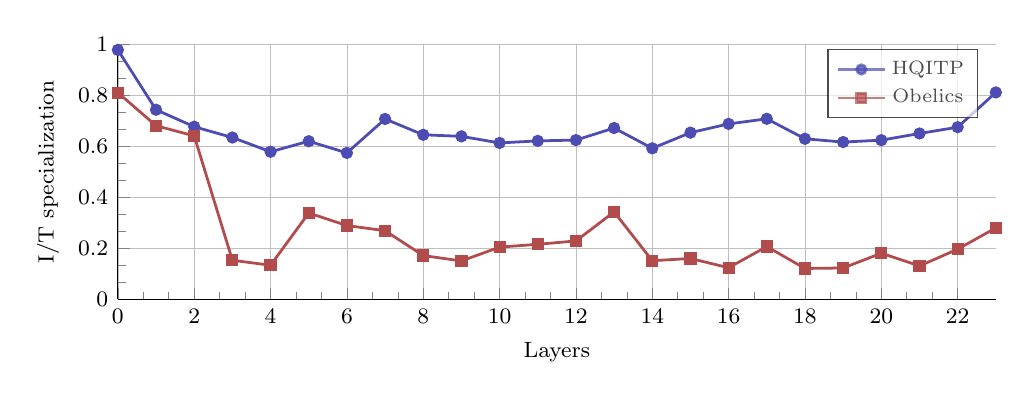
\begin{tikzpicture}
\begin{axis}[
    grid=major,
    grid style={line width=.1pt, draw=gray!30},
    major grid style={line width=.2pt,draw=gray!50},
    minor tick num=2,
    axis x line*=bottom,
    axis y line*=left,
    xmin=0,
    xmax=23,
    ymin=0.0,
    ymax=1.0,
    height=1.9in,
    width=1.05\linewidth,
    ylabel style={align=center, font=\footnotesize},
    xlabel style={font=\footnotesize},
    ylabel=\footnotesize{I/T specialization},
    xlabel={\footnotesize{Layers}},
    ytick distance=0.2,
    yticklabel style={font=\footnotesize, /pgf/number format/fixed, /pgf/number format/precision=2},
    xticklabel style={font=\footnotesize},
    xtick={0,2,4,6,8,10,12,14,16,18,20,22},
    xticklabels={0,2,4,6,8,10,12,14,16,18,20,22},
    mark options={solid},
    legend style={cells={align=left}, font=\scriptsize, text=black, opacity=0.7},
]

\addplot[color=blue!40!gray, mark=*, mark size=1.7pt, line width=1pt] plot coordinates {
(0, 0.9769479348349329)
(1, 0.7427025603097698)
(2, 0.6762374582380828)
(3, 0.6340138224507533)
(4, 0.5783047019889138)
(5, 0.6195673358863271)
(6, 0.5737861572855565)
(7, 0.7066104505575633)
(8, 0.6446960774170309)
(9, 0.6386074080824291)
(10, 0.6128197724774395)
(11, 0.620867456928868)
(12, 0.6240480502092688)
(13, 0.6712385178771478)
(14, 0.591805441066985)
(15, 0.6531511085896324)
(16, 0.6873617200378165)
(17, 0.7072043647262733)
(18, 0.6290614078343542)
(19, 0.6162376387022552)
(20, 0.6237776803436119)
(21, 0.649774290665718)
(22, 0.6745086003424091)
(23, 0.810597818982423)
};
\addlegendentry{HQITP}

\addplot[color=red!40!gray, mark=square*, mark size=1.7pt, line width=1pt] plot coordinates {
(0, 0.8098464848229123)
(1, 0.6803114998878562)
(2, 0.640428138604904)
(3, 0.15356616480436047)
(4, 0.13402442087930844)
(5, 0.33860156581505885)
(6, 0.2894806232076399)
(7, 0.269278406260023)
(8, 0.17195894943324286)
(9, 0.15091557473173656)
(10, 0.2050356661788283)
(11, 0.21603190628094793)
(12, 0.22923064654990588)
(13, 0.34291773221125066)
(14, 0.15175535984919586)
(15, 0.16059145647036643)
(16, 0.12438172525723101)
(17, 0.20722842981400202)
(18, 0.12145399323126793)
(19, 0.12335098001817868)
(20, 0.1811717532056517)
(21, 0.13129565163316004)
(22, 0.19701360887683683)
(23, 0.28035775702112686)
};
\addlegendentry{Obelics}
\end{axis}

\end{tikzpicture}

\caption{\textbf{MoE 专门化.} 基于熵的图像/文本专门化(见~\cref{sec:specialization})在两个数据源:HQITP 和 Obelics 的各层之间的变化。
\edit{两个数据源都表现出类似的趋势:在早期层中得分下降,随后在最后几层中再次上升.}}
\label{fig:tokens_specialization}

    \end{minipage}
    \vspace{3mm}
\end{figure}
